\documentclass[12pt,titlepage]{article}
\usepackage[letterpaper, left=1in, right=1in, top=1in, bottom=1in]{geometry}
\renewcommand{\baselinestretch}{2}
% \documentclass[10pt,titlepage,twocolumn]{article}
% \usepackage[letterpaper, left=0.75in, right=0.75in, top=0.75in, bottom=0.75in]{geometry}
% \renewcommand{\baselinestretch}{1.2}
\usepackage[T1]{fontenc}
% \usepackage[utf8]{inputenc}
\usepackage{csquotes}
\usepackage[english]{babel}
\usepackage{amscd,amssymb,amsmath,amsthm,mathtools}
\usepackage{kpfonts}
\usepackage{titling}
\usepackage{setspace}
\usepackage[sortcites=true]{biblatex}
\usepackage[inline]{enumitem}
\usepackage{siunitx}
\usepackage[skip=2pt]{caption}
\PassOptionsToPackage{hyphens}{url}\usepackage{hyperref}

\usepackage{tikz}
\usetikzlibrary{fadings}
\usetikzlibrary{patterns}
\usetikzlibrary{shadows.blur}
\usetikzlibrary{shapes}

% \pagenumbering{gobble}
\addbibresource{citations.bib}
\emergencystretch=1em

\title{\Large\textbf{Explaining and Evaluating the Use of RDMA in High Performance Containers} \\
Honors Computer Science Bachelor's Thesis}
\author{\textbf{Author}: Emerson Ford \\
\textbf{Advisor}: Dr.\ Ryan Stutsman \\
\textbf{Honors Faculty Advisor}: Dr.\ Tom Henderson \\
\textbf{Director of Undergraduate Studies}: Dr.\ James de St.\ Germain }
\date{\today}

\begin{document}
\maketitle


\section*{Abstract}
Containers are an increasingly popular packaging framework for complex applications, offering benefits such as lightweight isolation, portability, and ease of deployment.
These benefits have the potential to solve a myriad of issues that have long been present in the high performance computing world, presenting a compelling narrative for their use in these environments.
Unfortunately, standard container runtimes rely on relatively slow, virtualized network stacks to achieve network isolation and portability, which are incompatible with the kernel bypass networking technology RDMA\@.
This has limited the widespread adoption of containers in high performance computing environments where RDMA-reliant applications are quite common.

Recent projects such as FreeFlow and Mellanox's RDMA hardware have created solutions for enabling RDMA inside of containers while maintaining varying degrees of the benefits of standard containers.
However, despite the strong claims made by these solutions, many of their characteristics such as performance, isolation sacrifices, and scalability are either not well documented or simply not known; these characteristics being critical to assess for several high performance computing use cases.
This thesis attempts to remedy this issue by identifying, explaining, measuring, and comparing these characteristics for the various solutions available today for enabling RDMA in containers;
ultimately providing high performance computing end-users a more holistic perspective on which solutions may be most viable for their environment and use case.

\section{Introduction}
Containers offer a promising solution to a host of issues that have long plagued the high performance computing (HPC) world from dependency management to portable and reproducible environments to even lightweight sharing of hardware resources;
all of which being achieved through the use of statically built images and standardized container runtimes~\cite{containershpc}.
For users, cluster administrators, and application developers, this would provide more freedom and ease in application development and deployment as it eliminates the burden of working around the hundreds of possible environments on which the application may be deployed.
In addition, this also opens the door for easy migration and utilization of new, ``container first'' HPC platforms such as the cloud, Kubernetes, and SLATE that offer new compute and scheduling capabilities~\cite{slatepaper}.

However, despite these numerous benefits, the adoption of containers in the HPC world has been notably slow~\cite{hpcappscontainers}.
Among other issues like the until-recent lack of rootless container runtimes, standard container network stacks do not support Remote Direct Memory Access (RDMA), a networking technology that provides extremely low latency and high throughput with minimal CPU overhead by offloading memory accesses from the CPU to NIC hardware (hence the term ``kernel bypass networking'')~\cite{mellanoxrocerdmabenefits}.
This lack of support heavily restricts the use of native containers in HPC environments as trends like disaggregated storage, multi-machine workloads, and increased use of parallel libraries such as MPI have necessitated the use of high performance networking like RDMA to maintain performance.
To make the lack of RDMA support even worse, standard container network stacks by themselves have been shown to be both CPU intensive and significantly reduce container networking performance~\cite{abbasi2019performance,xavier2013performance,lee2018impact,zhao2017performance,kapovcius2020performance}, further worsening the networking downsides of containers in HPC environments.

Unfortunately, enabling support for RDMA in containers (and fast networking as a whole) is a nontrivial task.
Container runtimes rely on ``virtualized'' network stacks for creating flexible network overlays, enforcing isolation, and providing portability~\cite{xavier2013performance}.
These network stacks have, for the most part, only been expressible through software layers provided by the host kernel, adding significant software overhead to the processing of all network packets originating from and destined to containers.
Due to this, these network stacks are fundamentally incompatible with RDMA which requires bypassing the host kernel entirely for its performance guarantees.

While it is possible to run containers without container networking by exposing the host's NIC directly to running containers (a mode called ``host networking''), this comes with several notable disadvantages:
\begin{enumerate*}[label={(\arabic*)},itemjoin*={{, and }},itemjoin={{, }}]
	\item controlling fair sharing of the RDMA-capable NIC between multiple containers cannot be done programmatically
	\item containers are not relocatable/portable across multiple hosts
	\item common container orchestration tools like Kubernetes cannot be used
	\item network isolation and network routing policies for containers is disabled
\end{enumerate*}.
Thus, while this mode may be a viable for some environments, it is not adequate for the vast majority of container environments --- such as those that utilize Kubernetes heavily --- and additional solutions for enabling RDMA in containers are still needed.

Multiple groups have recently developed solutions for enabling RDMA in containers, each with certain sacrifices in container and/or RDMA guarantees to overcome this incompatibility.
The challenge is then to determine which solution (and subsequent sacrifices in guarantees) works best for a given environment.
This is the core problem this thesis seeks to address.
It is currently unnecessarily difficult to pick a solution due to a lack of exhaustive performance data and thorough explanations on exactly which guarantees are sacrificed for these various solutions.
This information is critical in HPC environments as applications may heavily rely on RDMA's low latency and/or high throughput guarantees; similarly, container security and isolation guarantees may be a requirement for those HPC environments that are multi-tenant or are running untrusted applications.

Therefore, this thesis will analyze multiple properties of the several solutions available today for enabling RDMA in containers, such as SoftRoCE~\cite{pandeysroce}, Shared HCA, SR-IOV~\cite{mellanoxdockerroce}, FreeFlow~\cite{kim2019freeflow}, and MasQ~\cite{he2020masq};
these properties being grouped in two main categories:

\noindent
\textbf{Container RDMA Network Properties:}
\begin{itemize}[nolistsep]
	% todo: reiterate what container IP means, should be the IP is not exposed to the network? not sure, this overlaps
	% with network pressure perhaps
	% maybe clarify this is intra-machine network isolation; external view and internal view? 
	\item \textit{Network Isolation}: each container has its own interface, routing tables, and network policies (also known as a network namespace); further, a container's IP should not inherently depend on the underlying NIC's network
	\item \textit{Controllability}: enforcing routing policies and traffic shaping on a container with an RDMA-capable NIC
		% maybe clarify this is host resource utilization
	\item \textit{Resource Utilization}: container networks should not be CPU or memory intensive
\end{itemize}

\noindent
\textbf{RDMA Properties:}
\begin{itemize}[nolistsep]
	\item \textit{Throughput}: how closely can a solution match host RDMA throughput
	\item \textit{Latency}: what latency overhead is incurred per message for a given solution
\end{itemize}

\noindent
and analyzed with varying levels of:
\begin{itemize}[nolistsep]
	\item number of virtualized RDMA devices on the cluster and host (e.g.\ where each virtualized RDMA device is allocated to a single container)
	\item message size of network payloads
\end{itemize}
which should adequately test the scalability of these properties.
Finally, comments will also be made on:
\begin{itemize}[nolistsep]
	\item \textit{Scalability Limits}: are there any other hardware or software limits on the NIC for scalability
	\item \textit{Proprietary}: can a solution be used across various RDMA-capable NIC vendors
	\item \textit{Maturity}: what support exists for a solution, how well tested is a solution
	\item \textit{Ease in Deployment}: are application changes necessary for a solution, how difficult is it to deploy the solution
	\item \textit{Execution Privileges}: can the solution be used without elevated capabilities such as \texttt{CAP\_SYS\_ADMIN}
	\item \textit{Network Pressure}: what additional pressure do these solutions put on the network
\end{itemize}
to assist in determining if a given environment can even support a given solution.

Additionally, these solutions can be generalized to three implementations: pure software, paravirtualization-like, and pure hardware;
with each solution in an implementation likely having similar properties.
Thus, this thesis should also provide general insight as to which implementations may be best suited for a given HPC environment.

% TODO: Add summary of conclusion here.

\section{Background}
\subsection{Networking Planes}\label{subsec:Networking Planes}
The state and logic of networking operations can be generally abstracted into three planes: the control plane, the data plane, and the management plane.
Understanding this abstraction is vital for understanding how these various RDMA in container solutions operate and why they exhibit their specific performance characteristics.

The \textit{control plane} handles the rules of how and to where network packets are forwarded.
Operations such as initiating connections, terminating connections, and connection resource management are considered as part of control plane operations and policies such as firewalls, routing policies and tables, traffic shaping, and interface properties (e.g.\ IP addresses) are considered as part of control plane policies.
It is desirable to have the control plane be highly flexible and configurable to allow for a wide expression of network topologies.

The \textit{data plane}, also known as the forwarding plane, handles the actual transmission of network data based on the configured logic of the control plane.
Operations such as memory copies into network buffers and packet transmission over the wire are considered as part of data plane operations and policies such as the size of network buffers are considered as part of data plane policies.
It is desirable to keep the data plane as low overhead as possible as overhead in the data plane has a significant impact on network performance due to every byte of a packet having to traverse the data plane.
Notably, it is the data plane that handles the ``execution'' of control plane policies, thus the control plane is only as expressive as the data plane allows.

The \textit{management plane} handles the configuration of the control plane and data plane policies.
Its operations consists primarily of using software tools such as the iproute2 collection of tools, \texttt{iptables} / \texttt{nftables}, \texttt{DHCP}, and \texttt{ovs-vsctl} that take input to reconfigure the specified plane's policies.
The management plane's policies primarily consist of security; specifically, defining who has access to use its tools, with what capabilities, and in what contexts.

In traditional host networking, the control plane and the data plane\footnote{barring the actual transmission on the wire which the NIC handles} exist as software in the kernel.
This provides an extremely high degree of flexibility and configurability for the control plane and data plane, but it results in the kernel being interposed in every networking operation.
As a result, this incurs performance penalties from the overhead of context switches, memory copies from user-space to kernel-space (or from RAM to CPU to the network device), and from simply being software (i.e.\ not being hardware accelerated or run on FPGAs).
On top of this, use of standard network protocols like TCP may exacerbate the performance penalties due to higher code complexity, built in retries and throttling, and protocol header overhead.

\subsection{RDMA Protocol}\label{subsec:RDMA Protocol}
Remote Direct Memory Access (RDMA) is an aptly named network protocol designed for the direct reading and writing of the memory of remote hosts with extremely low latency, high bandwidth, and minimal CPU overhead.
Support for it has been added to a number of parallel applications and libraries, such as TensorFlow and OpenMPI, and has seen wide spread adoption in the high performance computing world where it is run on top of either Infiniband or Ethernet~\cite{kim2019freeflow}.
At its core, RDMA is a form of kernel-bypass networking in that it shifts almost all of the data plane and control plane from the kernel to a combination of user-space and the network card.
While this eliminates most of the control plane and data plane configurability provided by the kernel, it provides substantial improvements in network latency and bandwidth.
For example, current top-of-the-line RDMA enabled NICs are capable of achieving sub-1\si{\micro\second} latency with >100Gb/s flows, performance not possible with even the most aggressive tuning of the Linux networking stack~\cite{mellanoxcx6doc,cloudflarelowlatency,intel800nic}.

Understanding the data paths, architecture, and implementation of network planes for RDMA itself is critical for understanding how and why these various RDMA in containers solutions work and will therefore be explained.

% todo: add terminology section here
% There's the channel adapter (CA) / NIC / physical device.
% There's the RDMA device for the software abstraction over the hardware.
% network ports
% GID table entries
% interfaces on top of the physical devices

\subsubsection{Data Plane}
While traditional host networking relies on kernel syscalls and interrupts as a communication channel for signalling packet sends and receives, RDMA instead utilizes in-memory queues that live in regions of memory explicitly shared between the user-space process and the NIC\footnote{the NIC using IOMMU to directly access memory without CPU interposition} as its data plane communication channel.
A user-space process will write a \textit{work request} (WR) to the designated TX Queue to initiate a message\footnote{in contrast to TCP and UDP where the user-space process handles chunking a message into packets, RDMA operations post full messages and the NIC handles chunking the message into packets} send.
The NIC will spin-loop on these shared-memory queues to detect when a work request has been posted.
Inside of this work request will be a fat pointer\footnote{fat pointers being a pointer with extent information} to another region of shared memory --- this being the actual message payload.
The NIC will consume the posted work request, read the payload directly from memory (a process known as Direct Memory Access or DMA), then transmit the payload over the wire, all without any kernel or CPU interposition.
The user-space process is then notified of whether that message send succeeded or not by a \textit{completion queue event} (CQE) that is posted by the NIC to the designated Completion Queue.

Following this, a user-space process can receive messages by posting a \textit{receive request} (RR) to the designated RX Queue, with these requests containing fat pointers to writable buffers in shared memory.
Only after a receive request with a memory buffer large enough has been posted will a NIC accept an incoming message.
When an incoming message is accepted, the NIC will similarly write the incoming payload to the specified shared-memory buffer found in the receive request~\cite{rdmaawareprogramming}.

It is worth noting that what is described above is technically considered \textit{two-sided} RDMA operations (these use the verbiage \textit{send} and \textit{receive}).
RDMA is also capable of \textit{one-sided} operations that consist of directly reading and writing the memory of the remote host (these use the verbiage \textit{write} and \textit{read}) without the remote host being involved in or aware of such operations, i.e.\ the remote user-space process does not need to post receive requests.
These one-sided operations follow a nearly identical data path to two-sided operations, minus the need for the RX Queue.

\begin{figure}
	\resizebox{\linewidth}{!}{
		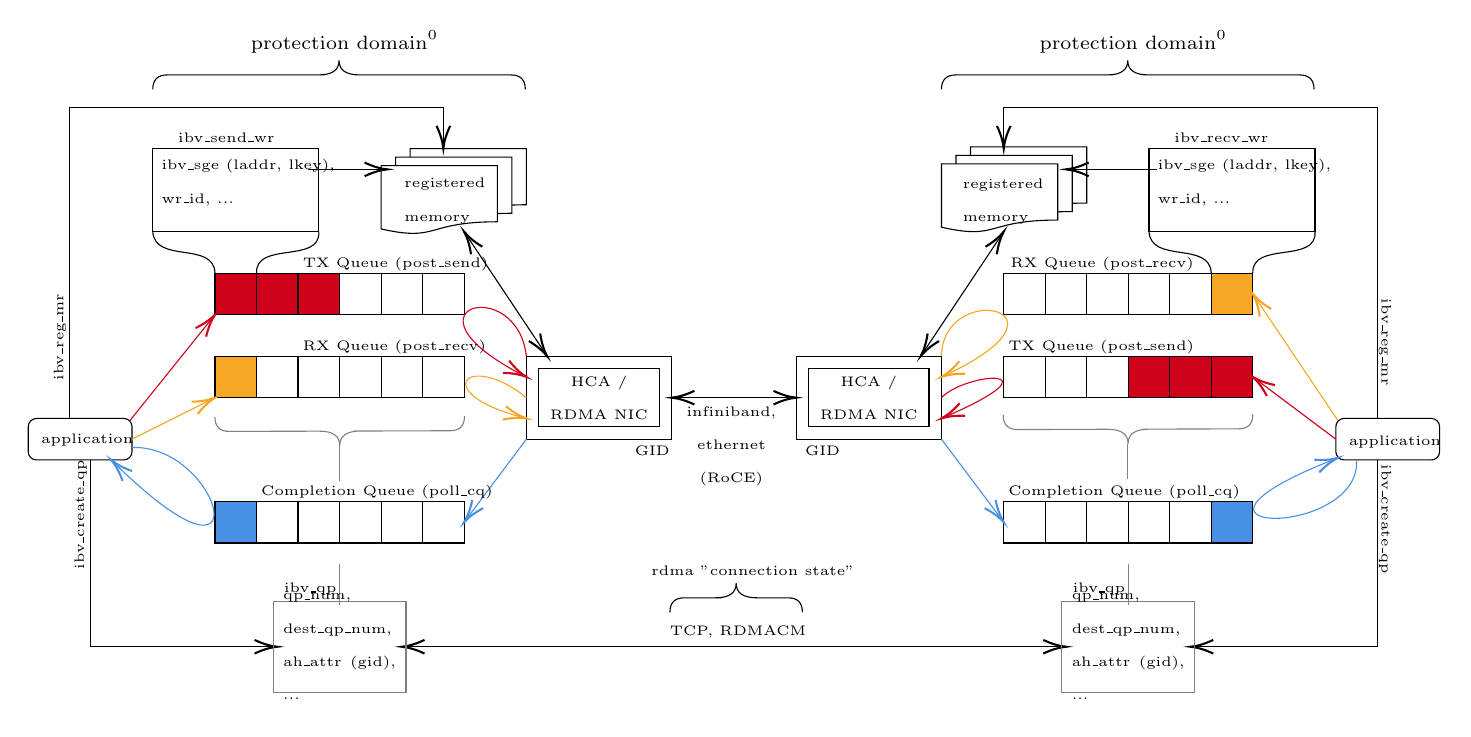
\begin{tikzpicture}[x=0.75pt,y=0.75pt,yscale=-1,xscale=1]
			\tikzset{every picture/.style={line width=0.75pt}} %set default line width to 0.75pt
%uncomment if require: \path (0,337); %set diagram left start at 0, and has height of 337

%Shape: Grid [id:dp4295659866532805]
\draw  [draw opacity=0] (100,220) -- (220,220) -- (220,240) -- (100,240) -- cycle ; \draw   (120,220) -- (120,240)(140,220) -- (140,240)(160,220) -- (160,240)(180,220) -- (180,240)(200,220) -- (200,240) ; \draw    ; \draw   (100,220) -- (220,220) -- (220,240) -- (100,240) -- cycle ;
%Shape: Grid [id:dp8946879606396433]
\draw  [draw opacity=0] (100,150) -- (220,150) -- (220,170) -- (100,170) -- cycle ; \draw   (120,150) -- (120,170)(140,150) -- (140,170)(160,150) -- (160,170)(180,150) -- (180,170)(200,150) -- (200,170) ; \draw    ; \draw   (100,150) -- (220,150) -- (220,170) -- (100,170) -- cycle ;
%Shape: Grid [id:dp4368011626744822]
\draw  [draw opacity=0] (100,110) -- (220,110) -- (220,130) -- (100,130) -- cycle ; \draw   (120,110) -- (120,130)(140,110) -- (140,130)(160,110) -- (160,130)(180,110) -- (180,130)(200,110) -- (200,130) ; \draw    ; \draw   (100,110) -- (220,110) -- (220,130) -- (100,130) -- cycle ;
%Shape: Frame [id:dp0617244658145758]
\draw   (250,150) -- (320,150) -- (320,190) -- (250,190) -- cycle(314,156) -- (256,156) -- (256,184) -- (314,184) -- cycle ;
%Curve Lines [id:da5967844605583035]
\draw [color={rgb, 255:red, 208; green, 2; blue, 27 }  ,draw opacity=1 ]   (250,150) .. controls (245.42,109.8) and (184.41,126.63) .. (249.02,159.5) ;
\draw [shift={(250,160)}, rotate = 206.63] [color={rgb, 255:red, 208; green, 2; blue, 27 }  ,draw opacity=1 ][line width=0.75]    (10.93,-3.29) .. controls (6.95,-1.4) and (3.31,-0.3) .. (0,0) .. controls (3.31,0.3) and (6.95,1.4) .. (10.93,3.29)   ;
%Straight Lines [id:da3545614732130127]
\draw [color={rgb, 255:red, 74; green, 144; blue, 226 }  ,draw opacity=1 ]   (250,190) -- (221.2,228.4) ;
\draw [shift={(220,230)}, rotate = 306.87] [color={rgb, 255:red, 74; green, 144; blue, 226 }  ,draw opacity=1 ][line width=0.75]    (10.93,-3.29) .. controls (6.95,-1.4) and (3.31,-0.3) .. (0,0) .. controls (3.31,0.3) and (6.95,1.4) .. (10.93,3.29)   ;
%Curve Lines [id:da204421881230066]
\draw [color={rgb, 255:red, 245; green, 166; blue, 35 }  ,draw opacity=1 ]   (250,170) .. controls (221.78,146.98) and (202.19,167.58) .. (248.57,179.64) ;
\draw [shift={(250,180)}, rotate = 193.98] [color={rgb, 255:red, 245; green, 166; blue, 35 }  ,draw opacity=1 ][line width=0.75]    (10.93,-3.29) .. controls (6.95,-1.4) and (3.31,-0.3) .. (0,0) .. controls (3.31,0.3) and (6.95,1.4) .. (10.93,3.29)   ;
%Shape: Rectangle [id:dp7444892557504112]
\draw   (70,50) -- (150,50) -- (150,90) -- (70,90) -- cycle ;
%Curve Lines [id:da4358799403511109]
\draw    (100,110) .. controls (99.4,94.4) and (71,105.6) .. (70,90) ;
%Curve Lines [id:da04054970173393413]
\draw    (120,110) .. controls (119.4,94.4) and (151,105.6) .. (150,90) ;
%Shape: Rectangle [id:dp09447409855918232]
\draw  [fill={rgb, 255:red, 208; green, 2; blue, 27 }  ,fill opacity=1 ] (140,110) -- (160,110) -- (160,130) -- (140,130) -- cycle ;
%Shape: Rectangle [id:dp7954961531438973]
\draw  [fill={rgb, 255:red, 208; green, 2; blue, 27 }  ,fill opacity=1 ] (120,110) -- (140,110) -- (140,130) -- (120,130) -- cycle ;
%Shape: Rectangle [id:dp375729093280755]
\draw  [fill={rgb, 255:red, 245; green, 166; blue, 35 }  ,fill opacity=1 ] (100,150) -- (120,150) -- (120,170) -- (100,170) -- cycle ;
%Shape: Rectangle [id:dp7009688837706805]
\draw  [fill={rgb, 255:red, 208; green, 2; blue, 27 }  ,fill opacity=1 ] (100,110) -- (120,110) -- (120,130) -- (100,130) -- cycle ;
%Shape: Rectangle [id:dp4753240489158659]
\draw  [fill={rgb, 255:red, 74; green, 144; blue, 226 }  ,fill opacity=1 ] (100,220) -- (120,220) -- (120,240) -- (100,240) -- cycle ;
%Rounded Rect [id:dp7482108927478565]
\draw   (10,184) .. controls (10,181.79) and (11.79,180) .. (14,180) -- (56,180) .. controls (58.21,180) and (60,181.79) .. (60,184) -- (60,196) .. controls (60,198.21) and (58.21,200) .. (56,200) -- (14,200) .. controls (11.79,200) and (10,198.21) .. (10,196) -- cycle ;
%Straight Lines [id:da0860623165459462]
\draw [color={rgb, 255:red, 208; green, 2; blue, 27 }  ,draw opacity=1 ]   (59,181) -- (98.75,131.56) ;
\draw [shift={(100,130)}, rotate = 488.8] [color={rgb, 255:red, 208; green, 2; blue, 27 }  ,draw opacity=1 ][line width=0.75]    (10.93,-3.29) .. controls (6.95,-1.4) and (3.31,-0.3) .. (0,0) .. controls (3.31,0.3) and (6.95,1.4) .. (10.93,3.29)   ;
%Straight Lines [id:da10819672911414313]
\draw [color={rgb, 255:red, 245; green, 166; blue, 35 }  ,draw opacity=1 ]   (60,190) -- (98.21,170.89) ;
\draw [shift={(100,170)}, rotate = 513.4300000000001] [color={rgb, 255:red, 245; green, 166; blue, 35 }  ,draw opacity=1 ][line width=0.75]    (10.93,-3.29) .. controls (6.95,-1.4) and (3.31,-0.3) .. (0,0) .. controls (3.31,0.3) and (6.95,1.4) .. (10.93,3.29)   ;
%Curve Lines [id:da5396028508269919]
\draw [color={rgb, 255:red, 74; green, 144; blue, 226 }  ,draw opacity=1 ]   (60,194) .. controls (102.79,192.41) and (125.18,273.98) .. (51.12,201.11) ;
\draw [shift={(50,200)}, rotate = 404.77] [color={rgb, 255:red, 74; green, 144; blue, 226 }  ,draw opacity=1 ][line width=0.75]    (10.93,-3.29) .. controls (6.95,-1.4) and (3.31,-0.3) .. (0,0) .. controls (3.31,0.3) and (6.95,1.4) .. (10.93,3.29)   ;
%Flowchart: Multidocument [id:dp5721236644573098]
\draw  [fill={rgb, 255:red, 255; green, 255; blue, 255 }  ,fill opacity=1 ] (194,50) -- (250,50) -- (250,77.06) .. controls (215,77.06) and (222,86.82) .. (194,80.5) -- cycle ; \draw  [fill={rgb, 255:red, 255; green, 255; blue, 255 }  ,fill opacity=1 ] (187,54.1) -- (243,54.1) -- (243,81.16) .. controls (208,81.16) and (215,90.92) .. (187,84.6) -- cycle ; \draw  [fill={rgb, 255:red, 255; green, 255; blue, 255 }  ,fill opacity=1 ] (180,58.2) -- (236,58.2) -- (236,85.26) .. controls (201,85.26) and (208,95.02) .. (180,88.7) -- cycle ;
%Straight Lines [id:da6912345896218269]
\draw    (145,60) -- (181,60) ;
\draw [shift={(183,60)}, rotate = 180] [color={rgb, 255:red, 0; green, 0; blue, 0 }  ][line width=0.75]    (10.93,-3.29) .. controls (6.95,-1.4) and (3.31,-0.3) .. (0,0) .. controls (3.31,0.3) and (6.95,1.4) .. (10.93,3.29)   ;
%Shape: Grid [id:dp119026641862925]
\draw  [draw opacity=0] (480,220) -- (600,220) -- (600,240) -- (480,240) -- cycle ; \draw   (500,220) -- (500,240)(520,220) -- (520,240)(540,220) -- (540,240)(560,220) -- (560,240)(580,220) -- (580,240) ; \draw    ; \draw   (480,220) -- (600,220) -- (600,240) -- (480,240) -- cycle ;
%Shape: Grid [id:dp0804991380561264]
\draw  [draw opacity=0] (480,150) -- (600,150) -- (600,170) -- (480,170) -- cycle ; \draw   (500,150) -- (500,170)(520,150) -- (520,170)(540,150) -- (540,170)(560,150) -- (560,170)(580,150) -- (580,170) ; \draw    ; \draw   (480,150) -- (600,150) -- (600,170) -- (480,170) -- cycle ;
%Shape: Grid [id:dp11715394785996025]
\draw  [draw opacity=0] (480,110) -- (600,110) -- (600,130) -- (480,130) -- cycle ; \draw   (500,110) -- (500,130)(520,110) -- (520,130)(540,110) -- (540,130)(560,110) -- (560,130)(580,110) -- (580,130) ; \draw    ; \draw   (480,110) -- (600,110) -- (600,130) -- (480,130) -- cycle ;
%Shape: Frame [id:dp8132523520793834]
\draw   (380,150) -- (450,150) -- (450,190) -- (380,190) -- cycle(444,156) -- (386,156) -- (386,184) -- (444,184) -- cycle ;
%Shape: Rectangle [id:dp9806953964426239]
\draw   (549.98,50) -- (629.98,50) -- (629.98,90) -- (549.98,90) -- cycle ;
%Curve Lines [id:da8538159727708337]
\draw    (579.98,110) .. controls (579.38,94.4) and (550.98,105.6) .. (549.98,90) ;
%Curve Lines [id:da503262725402064]
\draw    (599.98,110) .. controls (599.38,94.4) and (630.98,105.6) .. (629.98,90) ;
%Shape: Rectangle [id:dp23358801131092133]
\draw  [fill={rgb, 255:red, 208; green, 2; blue, 27 }  ,fill opacity=1 ] (580,150) -- (600,150) -- (600,170) -- (580,170) -- cycle ;
%Shape: Rectangle [id:dp16921311873779]
\draw  [fill={rgb, 255:red, 208; green, 2; blue, 27 }  ,fill opacity=1 ] (560,150) -- (580,150) -- (580,170) -- (560,170) -- cycle ;
%Shape: Rectangle [id:dp1685110147344583]
\draw  [fill={rgb, 255:red, 245; green, 166; blue, 35 }  ,fill opacity=1 ] (580,110) -- (600,110) -- (600,130) -- (580,130) -- cycle ;
%Shape: Rectangle [id:dp5932409601304787]
\draw  [fill={rgb, 255:red, 208; green, 2; blue, 27 }  ,fill opacity=1 ] (540,150) -- (560,150) -- (560,170) -- (540,170) -- cycle ;
%Shape: Rectangle [id:dp5864080847756401]
\draw  [fill={rgb, 255:red, 74; green, 144; blue, 226 }  ,fill opacity=1 ] (580,220) -- (600,220) -- (600,240) -- (580,240) -- cycle ;
%Rounded Rect [id:dp9740510619526319]
\draw   (640,184) .. controls (640,181.79) and (641.79,180) .. (644,180) -- (686,180) .. controls (688.21,180) and (690,181.79) .. (690,184) -- (690,196) .. controls (690,198.21) and (688.21,200) .. (686,200) -- (644,200) .. controls (641.79,200) and (640,198.21) .. (640,196) -- cycle ;
%Straight Lines [id:da16241601875679856]
\draw [color={rgb, 255:red, 208; green, 2; blue, 27 }  ,draw opacity=1 ]   (640,190) -- (601.6,161.2) ;
\draw [shift={(600,160)}, rotate = 396.87] [color={rgb, 255:red, 208; green, 2; blue, 27 }  ,draw opacity=1 ][line width=0.75]    (10.93,-3.29) .. controls (6.95,-1.4) and (3.31,-0.3) .. (0,0) .. controls (3.31,0.3) and (6.95,1.4) .. (10.93,3.29)   ;
%Straight Lines [id:da918563124412445]
\draw [color={rgb, 255:red, 245; green, 166; blue, 35 }  ,draw opacity=1 ]   (641,181) -- (601.12,121.66) ;
\draw [shift={(600,120)}, rotate = 416.09000000000003] [color={rgb, 255:red, 245; green, 166; blue, 35 }  ,draw opacity=1 ][line width=0.75]    (10.93,-3.29) .. controls (6.95,-1.4) and (3.31,-0.3) .. (0,0) .. controls (3.31,0.3) and (6.95,1.4) .. (10.93,3.29)   ;
%Curve Lines [id:da07688196394851687]
\draw [color={rgb, 255:red, 74; green, 144; blue, 226 }  ,draw opacity=1 ]   (650,200) .. controls (652.32,238.47) and (544.75,236.69) .. (639.56,199.56) ;
\draw [shift={(641,199)}, rotate = 518.8399999999999] [color={rgb, 255:red, 74; green, 144; blue, 226 }  ,draw opacity=1 ][line width=0.75]    (10.93,-3.29) .. controls (6.95,-1.4) and (3.31,-0.3) .. (0,0) .. controls (3.31,0.3) and (6.95,1.4) .. (10.93,3.29)   ;
%Flowchart: Multidocument [id:dp24323844239769876]
\draw  [fill={rgb, 255:red, 255; green, 255; blue, 255 }  ,fill opacity=1 ] (464,49.17) -- (520,49.17) -- (520,76.23) .. controls (485,76.23) and (492,85.99) .. (464,79.67) -- cycle ; \draw  [fill={rgb, 255:red, 255; green, 255; blue, 255 }  ,fill opacity=1 ] (457,53.27) -- (513,53.27) -- (513,80.33) .. controls (478,80.33) and (485,90.09) .. (457,83.77) -- cycle ; \draw  [fill={rgb, 255:red, 255; green, 255; blue, 255 }  ,fill opacity=1 ] (450,57.37) -- (506,57.37) -- (506,84.43) .. controls (471,84.43) and (478,94.19) .. (450,87.87) -- cycle ;
%Straight Lines [id:da7059822979397073]
\draw    (660,180) -- (660,30) ;
%Straight Lines [id:da481201579183531]
\draw    (512,60) -- (554,60) ;
\draw [shift={(510,60)}, rotate = 0] [color={rgb, 255:red, 0; green, 0; blue, 0 }  ][line width=0.75]    (10.93,-3.29) .. controls (6.95,-1.4) and (3.31,-0.3) .. (0,0) .. controls (3.31,0.3) and (6.95,1.4) .. (10.93,3.29)   ;
%Straight Lines [id:da22589634957435445]
\draw [color={rgb, 255:red, 0; green, 0; blue, 0 }  ,draw opacity=1 ]   (322,170) -- (378,170) ;
\draw [shift={(380,170)}, rotate = 180] [color={rgb, 255:red, 0; green, 0; blue, 0 }  ,draw opacity=1 ][line width=0.75]    (10.93,-3.29) .. controls (6.95,-1.4) and (3.31,-0.3) .. (0,0) .. controls (3.31,0.3) and (6.95,1.4) .. (10.93,3.29)   ;
\draw [shift={(320,170)}, rotate = 0] [color={rgb, 255:red, 0; green, 0; blue, 0 }  ,draw opacity=1 ][line width=0.75]    (10.93,-3.29) .. controls (6.95,-1.4) and (3.31,-0.3) .. (0,0) .. controls (3.31,0.3) and (6.95,1.4) .. (10.93,3.29)   ;
%Straight Lines [id:da11720587390108372]
\draw    (192,290) -- (508,290) ;
\draw [shift={(510,290)}, rotate = 180] [color={rgb, 255:red, 0; green, 0; blue, 0 }  ][line width=0.75]    (10.93,-3.29) .. controls (6.95,-1.4) and (3.31,-0.3) .. (0,0) .. controls (3.31,0.3) and (6.95,1.4) .. (10.93,3.29)   ;
\draw [shift={(190,290)}, rotate = 0] [color={rgb, 255:red, 0; green, 0; blue, 0 }  ][line width=0.75]    (10.93,-3.29) .. controls (6.95,-1.4) and (3.31,-0.3) .. (0,0) .. controls (3.31,0.3) and (6.95,1.4) .. (10.93,3.29)   ;
%Curve Lines [id:da21032506501189785]
\draw [color={rgb, 255:red, 245; green, 166; blue, 35 }  ,draw opacity=1 ]   (450,150) .. controls (450.6,112.59) and (520.69,127.45) .. (451.06,159.52) ;
\draw [shift={(450,160)}, rotate = 335.59000000000003] [color={rgb, 255:red, 245; green, 166; blue, 35 }  ,draw opacity=1 ][line width=0.75]    (10.93,-3.29) .. controls (6.95,-1.4) and (3.31,-0.3) .. (0,0) .. controls (3.31,0.3) and (6.95,1.4) .. (10.93,3.29)   ;
%Curve Lines [id:da1795237296648432]
\draw [color={rgb, 255:red, 208; green, 2; blue, 27 }  ,draw opacity=1 ]   (450,170) .. controls (461.68,157.72) and (508.84,154.46) .. (451.76,179.24) ;
\draw [shift={(450,180)}, rotate = 336.82] [color={rgb, 255:red, 208; green, 2; blue, 27 }  ,draw opacity=1 ][line width=0.75]    (10.93,-3.29) .. controls (6.95,-1.4) and (3.31,-0.3) .. (0,0) .. controls (3.31,0.3) and (6.95,1.4) .. (10.93,3.29)   ;
%Straight Lines [id:da2007010103317477]
\draw [color={rgb, 255:red, 74; green, 144; blue, 226 }  ,draw opacity=1 ]   (450,190) -- (478.8,228.4) ;
\draw [shift={(480,230)}, rotate = 233.13] [color={rgb, 255:red, 74; green, 144; blue, 226 }  ,draw opacity=1 ][line width=0.75]    (10.93,-3.29) .. controls (6.95,-1.4) and (3.31,-0.3) .. (0,0) .. controls (3.31,0.3) and (6.95,1.4) .. (10.93,3.29)   ;
%Shape: Brace [id:dp9940577590245101]
\draw   (383,273.42) .. controls (383,268.75) and (380.67,266.42) .. (376,266.42) -- (361.08,266.42) .. controls (354.41,266.42) and (351.08,264.09) .. (351.08,259.42) .. controls (351.08,264.09) and (347.75,266.42) .. (341.08,266.42)(344.08,266.42) -- (326.17,266.42) .. controls (321.5,266.42) and (319.17,268.75) .. (319.17,273.42) ;
%Straight Lines [id:da4361920428251189]
\draw    (660,200) -- (660,290) ;
%Straight Lines [id:da480314407062288]
\draw    (40,200) -- (40,290) ;
%Shape: Brace [id:dp588298908527398]
\draw  [color={rgb, 255:red, 128; green, 128; blue, 128 }  ,draw opacity=1 ] (99.93,179.28) .. controls (99.95,183.95) and (102.29,186.27) .. (106.96,186.26) -- (150.09,186.13) .. controls (156.76,186.1) and (160.1,188.42) .. (160.11,193.09) .. controls (160.1,188.42) and (163.42,186.08) .. (170.09,186.06)(167.09,186.07) -- (213.22,185.93) .. controls (217.89,185.92) and (220.21,183.58) .. (220.2,178.91) ;
%Straight Lines [id:da0889380362629657]
\draw    (40,290) -- (128,290) ;
\draw [shift={(130,290)}, rotate = 180] [color={rgb, 255:red, 0; green, 0; blue, 0 }  ][line width=0.75]    (10.93,-3.29) .. controls (6.95,-1.4) and (3.31,-0.3) .. (0,0) .. controls (3.31,0.3) and (6.95,1.4) .. (10.93,3.29)   ;
%Straight Lines [id:da17063350648323872]
\draw [color={rgb, 255:red, 128; green, 128; blue, 128 }  ,draw opacity=1 ]   (160,193) -- (160,210) ;
%Straight Lines [id:da735591769614332]
\draw [color={rgb, 255:red, 128; green, 128; blue, 128 }  ,draw opacity=1 ]   (160,250) -- (160,270) ;
%Shape: Brace [id:dp7463787220884971]
\draw  [color={rgb, 255:red, 128; green, 128; blue, 128 }  ,draw opacity=1 ] (479.73,178.38) .. controls (479.75,183.05) and (482.09,185.37) .. (486.76,185.36) -- (529.89,185.22) .. controls (536.56,185.2) and (539.9,187.52) .. (539.91,192.19) .. controls (539.9,187.52) and (543.22,185.18) .. (549.89,185.16)(546.89,185.17) -- (593.02,185.02) .. controls (597.69,185.01) and (600.01,182.67) .. (600,178) ;
%Straight Lines [id:da6347067855883498]
\draw [color={rgb, 255:red, 128; green, 128; blue, 128 }  ,draw opacity=1 ]   (539.8,192.09) -- (539.8,209.09) ;
%Straight Lines [id:da7879312663238379]
\draw [color={rgb, 255:red, 128; green, 128; blue, 128 }  ,draw opacity=1 ]   (540,250) -- (540,270) ;
%Straight Lines [id:da34735570105619973]
\draw    (660,290) -- (572,290) ;
\draw [shift={(570,290)}, rotate = 360] [color={rgb, 255:red, 0; green, 0; blue, 0 }  ][line width=0.75]    (10.93,-3.29) .. controls (6.95,-1.4) and (3.31,-0.3) .. (0,0) .. controls (3.31,0.3) and (6.95,1.4) .. (10.93,3.29)   ;
%Straight Lines [id:da6922947722733842]
\draw    (480,30) -- (660,30) ;
%Straight Lines [id:da8214317936198106]
\draw    (480,30) -- (480,48) ;
\draw [shift={(480,50)}, rotate = 270] [color={rgb, 255:red, 0; green, 0; blue, 0 }  ][line width=0.75]    (10.93,-3.29) .. controls (6.95,-1.4) and (3.31,-0.3) .. (0,0) .. controls (3.31,0.3) and (6.95,1.4) .. (10.93,3.29)   ;
%Straight Lines [id:da3127224438135543]
\draw    (30,180) -- (30,30) ;
%Straight Lines [id:da25223149816814294]
\draw    (30,30) -- (210,30) ;
%Straight Lines [id:da6150923577431217]
\draw    (210,30) -- (210,48) ;
\draw [shift={(210,50)}, rotate = 270] [color={rgb, 255:red, 0; green, 0; blue, 0 }  ][line width=0.75]    (10.93,-3.29) .. controls (6.95,-1.4) and (3.31,-0.3) .. (0,0) .. controls (3.31,0.3) and (6.95,1.4) .. (10.93,3.29)   ;
%Shape: Brace [id:dp7460733200764286]
\draw   (249.5,21.5) .. controls (249.5,16.83) and (247.17,14.5) .. (242.5,14.5) -- (169.75,14.5) .. controls (163.08,14.5) and (159.75,12.17) .. (159.75,7.5) .. controls (159.75,12.17) and (156.42,14.5) .. (149.75,14.5)(152.75,14.5) -- (77,14.5) .. controls (72.33,14.5) and (70,16.83) .. (70,21.5) ;
%Shape: Brace [id:dp25327117875899263]
\draw   (629.5,21.5) .. controls (629.5,16.83) and (627.17,14.5) .. (622.5,14.5) -- (549.75,14.5) .. controls (543.08,14.5) and (539.75,12.17) .. (539.75,7.5) .. controls (539.75,12.17) and (536.42,14.5) .. (529.75,14.5)(532.75,14.5) -- (457,14.5) .. controls (452.33,14.5) and (450,16.83) .. (450,21.5) ;
%Straight Lines [id:da5693657957631059]
\draw    (221.11,91.66) -- (258.89,148.34) ;
\draw [shift={(260,150)}, rotate = 236.31] [color={rgb, 255:red, 0; green, 0; blue, 0 }  ][line width=0.75]    (10.93,-3.29) .. controls (6.95,-1.4) and (3.31,-0.3) .. (0,0) .. controls (3.31,0.3) and (6.95,1.4) .. (10.93,3.29)   ;
\draw [shift={(220,90)}, rotate = 56.31] [color={rgb, 255:red, 0; green, 0; blue, 0 }  ][line width=0.75]    (10.93,-3.29) .. controls (6.95,-1.4) and (3.31,-0.3) .. (0,0) .. controls (3.31,0.3) and (6.95,1.4) .. (10.93,3.29)   ;
%Straight Lines [id:da648148726214795]
\draw    (478.89,91.66) -- (441.11,148.34) ;
\draw [shift={(440,150)}, rotate = 303.69] [color={rgb, 255:red, 0; green, 0; blue, 0 }  ][line width=0.75]    (10.93,-3.29) .. controls (6.95,-1.4) and (3.31,-0.3) .. (0,0) .. controls (3.31,0.3) and (6.95,1.4) .. (10.93,3.29)   ;
\draw [shift={(480,90)}, rotate = 123.69] [color={rgb, 255:red, 0; green, 0; blue, 0 }  ][line width=0.75]    (10.93,-3.29) .. controls (6.95,-1.4) and (3.31,-0.3) .. (0,0) .. controls (3.31,0.3) and (6.95,1.4) .. (10.93,3.29)   ;

% Text Node
\draw (121,211) node [anchor=north west][inner sep=0.75pt]  [font=\tiny] [align=left] {Completion Queue (poll\_cq)};
% Text Node
\draw (141,101) node [anchor=north west][inner sep=0.75pt]  [font=\tiny] [align=left] {TX Queue (post\_send)};
% Text Node
\draw (141,141) node [anchor=north west][inner sep=0.75pt]  [font=\tiny] [align=left] {RX Queue (post\_recv)};
% Text Node
\draw (81,41) node [anchor=north west][inner sep=0.75pt]  [font=\tiny] [align=left] {ibv\_send\_wr};
% Text Node
\draw (73,54) node [anchor=north west][inner sep=0.75pt]  [font=\tiny] [align=left] {ibv\_sge (laddr, lkey),\\wr\_id, ...};
% Text Node
\draw (15,186) node [anchor=north west][inner sep=0.75pt]  [font=\tiny] [align=left] {application};
% Text Node
\draw (190,63) node [anchor=north west][inner sep=0.75pt]  [font=\tiny] [align=left] {registered\\memory};
% Text Node
\draw (21,163) node [anchor=north west][inner sep=0.75pt]  [font=\tiny,rotate=-270] [align=left] {ibv\_reg\_mr};
% Text Node
\draw (481,141) node [anchor=north west][inner sep=0.75pt]  [font=\tiny] [align=left] {TX Queue (post\_send)};
% Text Node
\draw (482,101) node [anchor=north west][inner sep=0.75pt]  [font=\tiny] [align=left] {RX Queue (post\_recv)};
% Text Node
\draw (560.98,41) node [anchor=north west][inner sep=0.75pt]  [font=\tiny] [align=left] {ibv\_recv\_wr};
% Text Node
\draw (552.98,54) node [anchor=north west][inner sep=0.75pt]  [font=\tiny] [align=left] {ibv\_sge (laddr, lkey),\\wr\_id, ...};
% Text Node
\draw (645,187) node [anchor=north west][inner sep=0.75pt]  [font=\tiny] [align=left] {application};
% Text Node
\draw (459,63.17) node [anchor=north west][inner sep=0.75pt]  [font=\tiny] [align=left] {registered\\memory};
% Text Node
\draw (668,121) node [anchor=north west][inner sep=0.75pt]  [font=\tiny,rotate=-90] [align=left] {ibv\_reg\_mr};
% Text Node
\draw (321,173) node [anchor=north west][inner sep=0.75pt]  [font=\tiny] [align=left] {\begin{minipage}[lt]{39.83664400000001pt}\setlength\topsep{0pt}
\begin{center}
infiniband,\\ethernet (RoCE)
\end{center}

\end{minipage}};
% Text Node
\draw (481,211) node [anchor=north west][inner sep=0.75pt]  [font=\tiny] [align=left] {Completion Queue (poll\_cq)};
% Text Node
\draw (285,170) node  [font=\tiny] [align=left] {\begin{minipage}[lt]{39.440000000000005pt}\setlength\topsep{0pt}
\begin{center}
HCA /\\RDMA NIC
\end{center}

\end{minipage}};
% Text Node
\draw (415,170) node  [font=\tiny] [align=left] {\begin{minipage}[lt]{39.440000000000005pt}\setlength\topsep{0pt}
\begin{center}
HCA /\\RDMA NIC
\end{center}

\end{minipage}};
% Text Node
\draw (301,192) node [anchor=north west][inner sep=0.75pt]  [font=\tiny] [align=left] {GID};
% Text Node
\draw (383,192) node [anchor=north west][inner sep=0.75pt]  [font=\tiny] [align=left] {GID};
% Text Node
\draw  [color={rgb, 255:red, 128; green, 128; blue, 128 }  ,draw opacity=1 ]  (128,268) -- (192,268) -- (192,312) -- (128,312) -- cycle  ;
\draw (160,290) node  [font=\tiny] [align=left] {\begin{minipage}[lt]{40.800000000000004pt}\setlength\topsep{0pt}
qp\_num, dest\_qp\_num, ah\_attr (gid), ...
\end{minipage}};
% Text Node
\draw (132,258) node [anchor=north west][inner sep=0.75pt]  [font=\tiny] [align=left] {ibv\_qp};
% Text Node
\draw (309,250) node [anchor=north west][inner sep=0.75pt]  [font=\tiny] [align=left] {rdma "connection state"};
% Text Node
\draw (31,254) node [anchor=north west][inner sep=0.75pt]  [font=\tiny,rotate=-270] [align=left] {ibv\_create\_qp};
% Text Node
\draw (668,201) node [anchor=north west][inner sep=0.75pt]  [font=\tiny,rotate=-90] [align=left] {ibv\_create\_qp};
% Text Node
\draw (352,283) node  [font=\tiny] [align=left] {\begin{minipage}[lt]{68pt}\setlength\topsep{0pt}
\begin{center}
TCP, RDMACM
\end{center}

\end{minipage}};
% Text Node
\draw  [color={rgb, 255:red, 128; green, 128; blue, 128 }  ,draw opacity=1 ]  (508,268) -- (572,268) -- (572,312) -- (508,312) -- cycle  ;
\draw (540,290) node  [font=\tiny] [align=left] {\begin{minipage}[lt]{40.800000000000004pt}\setlength\topsep{0pt}
qp\_num, dest\_qp\_num, ah\_attr (gid), ...
\end{minipage}};
% Text Node
\draw (512,258) node [anchor=north west][inner sep=0.75pt]  [font=\tiny] [align=left] {ibv\_qp};
% Text Node
\draw (116,-8) node [anchor=north west][inner sep=0.75pt]  [font=\scriptsize] [align=left] {protection domain$\displaystyle ^{0}$};
% Text Node
\draw (496,-8) node [anchor=north west][inner sep=0.75pt]  [font=\scriptsize] [align=left] {protection domain$\displaystyle ^{0}$};

		\end{tikzpicture}
	}
	\caption{Diagram of RDMA's data paths}
\end{figure}

\subsubsection{Control Plane}\label{subsubsec:Control Plane}
With the data plane split between shared-memory and the NIC, it then follows that the majority of the RDMA control plane must also live between shared-memory and the NIC\@.
This, in conjunction with RDMA having a different implementation for each network fabric, results in the RDMA control plane having a radically different paradigm than that of traditional host networking.
Further, the RDMA control plane has the notion of both a \textit{device} and \textit{interface}, where the device is what is interacted with for RDMA operations and the interface is what the kernel provides on top of the NIC for standard network operations.
There are four key pieces that make up the RDMA control plane: the RDMA API library and device drivers, connection state, routing information, and interface management (i.e.\ multiplexing).

First, user-space processes utilize RDMA through a library known as \texttt{libibverbs}, which provides a central API for RDMA use regardless of network fabric~\cite{rdmacoredocumentation}.
This library handles both data plane operations, such as creating work requests or polling the completion queue, and control plane operations such as device metadata queries, queue creation and instantiation, or registration of shared memory with the NIC\@.
However, while data plane operations use the shared-memory regions as a communication channel, most control plane operations cannot do the same.
For example, these operations may involve the actual creation or manipulation of the shared memory region, or may be invoked when a shared memory region does not exist.
Thus, device drivers must be used as a communication channel for these operations.
This is, critically, one of two times the kernel is involved in RDMA operations.
Alongside \texttt{libibverbs} are drivers for the NIC itself;
these drivers expose character device files (usually in \texttt{/dev/infiniband} and/or \texttt{/sys/class/infiniband}) that user-space processes can interact with\footnote{usually with \texttt{read}, \texttt{write}, or \texttt{ioctl} syscalls, which is what results in the kernel / driver involvement} as a control plane communication channel to the NIC~\cite{linuxkernellibibverbs}.
Thus, all RDMA operations are initiated with \texttt{libibverbs}, which then feed into either shared memory for data plane operations or device drivers using character devices for control plane operations.
Note, these control plane operations tend to be so infrequent (e.g.\ most applications will use long running connections and thus will initiate connections rarely), the performance penalty of kernel interposition is negligible here.

\begin{figure}
	\centering
	\resizebox{0.8\linewidth}{!}{
		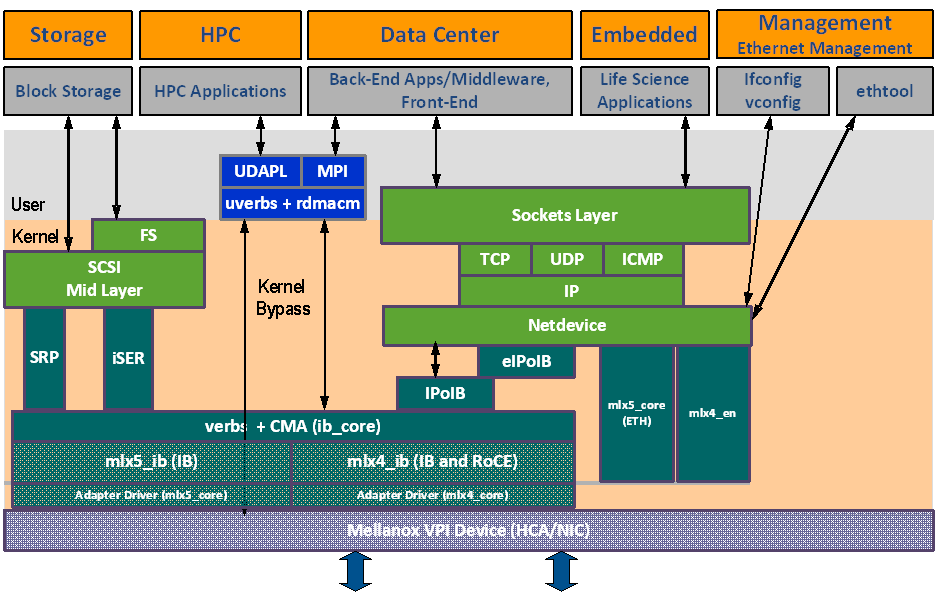
\includegraphics{libibverbsstack.png}
	}
	\caption{\texttt{libibverbs} stack}
	\caption*{Source:~\cite{mlnxofedmanual}}
\end{figure}

Second, RDMA maintains a notion of connection state, similar to that of TCP, stored in a structure known as \texttt{ibv\_qp}\@.
This structure contains fields such as \texttt{qp\_num}, \texttt{ibv\_device}, \texttt{dest\_qp\_num}, and \texttt{dlid} / \texttt{dgid}\footnote{there are Infiniband-specific layer-2 and layer-3 addresses respectively, however the \texttt{gid} can and is used to store MAC addresses, IPv4 addresses, and/or IPv6 addresses for Ethernet}.
These are, in respective order, analogous to local port, local IP, remote port, and remote IP in a TCP connection, and tell the NIC to which machine and to which receive queue on that machine all work requests in a specific TX queue should go to.
Further, this structure also contains fields such as \texttt{ibv\_pd} which specify which regions of shared memory a remote host can access using a set of generated cryptographic keys.

There is the question of how some of the state in this structure --- specifically \texttt{dest\_qp\_num}, \texttt{dlid} / \texttt{dgid}, pointers to remote memory, and the cryptographic keys for accessing those regions of remote memory --- is populated.
The RDMA protocol itself does not specify how to share this state and is thus deferred to standard networking facilities~\cite{rocev2spec}, this being the second time the kernel is involved in RDMA operations.
The user-space process can either manually populate and share this state over a standard protocol like TCP, or use the \texttt{rdmacm} facilities (having its own library and character devices) which handles the full creation of \texttt{ibv\_qp} using the most appropriate network protocol.
Once this state is populated, this structure is then registered with the NIC~\cite{rdmacoredocumentation,rdmacorerepo,rdmaawareprogramming}.

Third, RDMA-capable NICs are, first and foremost, standard NICs and thus have at least minimal support for routing capabilities.
On Ethernet fabrics, this means that at the hardware layer (ergo being exposed to the RDMA control plane) the RDMA-capable NIC has a MAC address and, in many cases, support for VLAN tagging.
These properties are used by the now outdated RDMA protocol RoCE v1, which allowed for RDMA over a single Ethernet broadcast domain.
Now, a MAC address alone does not suffice for standard networking, thus the host networking stack adds an IP layer on top of this for layer-3 routing.
Normally, this IP layer exists solely in the host's software, but drivers for the RDMA-capable Ethernet NICs have added functionality to expose IP addresses and VLAN tags to the NIC, which are then stored in the NIC's GID table.
These are then accessible to the RDMA control plane and are used by the RDMA protocol RoCE v2 that encapsulates RDMA packets inside of UDP packets for IP routable RDMA\@.
On Infiniband fabrics, the story is more straight forward.
In contrast to Ethernet NICs, most of the Infiniband networking logic lives on the NIC hardware (these Infiniband NICs being formally called HCAs), thus much of the Infiniband interface information --- such as its Local Identifier (LID), a layer-2 address, and Global Identifier (GID), a layer-3 address --- is stored on the NIC and is accessible to the RDMA control plane~\cite{mlnxofedmanual}.
However, for both Ethernet and Infiniband, next hop information (usually deduced with the subnet mask or Infiniband PathRecord) is not exposed by the kernel to the NIC\@.
As the final piece, user-space libraries (or the \texttt{rdmacm} module) will, depending on the specific NIC implementation, populate this information using the \texttt{ibv\_ah\_attr} and \texttt{ibv\_global\_route} structures, which are nested inside of \texttt{ibv\_qp}~\cite{rdmaawareprogramming,infinibandarch,rdmacorerepo}.

Support beyond these minimal routing capabilities for the RDMA control plane, such as firewalls at the host level and complex routing rules, is dependent on the features the NIC itself provides as these would have to be executed in the NIC's hardware.
This results in widely varying capabilities of the RDMA control plane depending on the NIC used --- a point that will be pertinent when discussing the various RDMA in container solutions.
Regardless, even if the NIC does not support some RDMA control plane functionality, an option may be to enforce it at the network level if the network fabric supports it.

Finally, RDMA-capable NICs tend to support the creation of multiple interfaces on top of a single NIC using both software and hardware based multiplexing.
The exact capabilities and functionality of this multiplexing is, again, dependent on what the NIC or NIC driver provides;
but, in general, software based multiplexing is managed by the kernel and integrates with the NIC using the aforementioned sharing and storage of IP addresses and VLAN tags to the NIC's GID table.
When a new interface or IP address assignment is created in the kernel (using commands like \texttt{ip addr add}), this creates a new entry in the NIC's GID table, which can then be used for both RDMA connection state sharing (using the kernel's interface abstraction), and for RDMA sends and receives (by specifying this new GID in the \texttt{ibv\_device} structure).
The scalability of this is, however, limited as the GID table has a fixed size in the NIC and with protocols like RoCEv2 requiring two GID entries minimum per interface, GID table entry exhaustion is a real possibility.

Hardware-based multiplexing, in general, uses Single Root I/O Virtualization (SR-IOV) which allows a single NIC (called the Physical Function or PF) to expose itself as multiple PCIe devices (each called a Virtual Function or VF).
These PCIe devices will appear as unique hardware network devices (as opposed to a software abstraction) to the kernel or hypervisor that can be handed out to individual virtual machines or isolated in namespaces.
On Ethernet, these VFs will appear as unique interfaces to the network, each with its own MAC address and, on some NICs, can have VLAN restrictions set on them by the host VM that cannot be overridden by the guest VM\@.
On Infiniband, the network is not made aware of each VF (formally called a vHCA), and the PF handles switching from the network fabric to each individual VF\@.
SR-IOV provides another form of virtualization, often useful in the context of virtual machines, but does suffer from hardware constraints as it relies on available hardware resources.
For example, the number of possible VFs is usually capped to under 150; use of VFs on Ethernet NICs can result in IP address exhaustion; and SR-IOV struggles with the same GID table entry exhaustion as software-based multiplexing as VFs share the same GID table as PFs, with GID table entry exhaustion resulting in the disabling of RDMA on some VFs~\cite{mlnxofedmanual}.

\subsubsection{Management Plane}\label{subsubsec:Management Plane}
The management plane for RDMA, which is integrated in the management plane for the NICs themselves, is then relatively straight forward.
Similar to control plane operations, character devices and device drivers are used as the communication channel for management plane operations, with libraries like \texttt{libibumad} being used to define the communication data types.
User tools like \texttt{ibstat} or \texttt{ibdiag}, as well as network managers like Infiniband's Subnet Manager, will use these libraries to reconfigure NIC policies.
These character devices can also be hidden from user-space processes as a method to prohibit NIC policy configuration.

Recently, RDMA-capable NIC device drivers have begun adding functionality to existing kernel systems to allow for minimal NIC and RDMA policy configuration with native OS tools like \texttt{devlink} and iproute2.
This has allowed for some native compatibility with existing kernel systems, like using capabilities to control IP assignment on RDMA-capable NICs~\cite{mlnxofedmanual}.
However, it still remains that the majority of the kernel's data plane and control plane systems, such as \texttt{iptables}/\texttt{nftables}/netfilter, are not exposed to the RDMA-capable NIC and are thus invalid in the context of RDMA operations.

\subsection{Containers}\label{subsec:Containers}
Containers are, as mentioned previously, a Linux-based packaging and deployment framework for complex applications.
Reminiscent of a unikernel, containers provide portable runtime environments, strong isolation, and fine grain access control to kernel resources for user-space processes.
These are accomplished with a combination of several Linux kernel systems.

First, for portable runtime environments.
Containers are bundled as \textit{container images}, which contains a file system\footnote{usually a union file system to allow for deduplication across multiple container images} that holds all runtime dependencies and binaries for the application, much like a static binary.
The kernel will then isolate the application process to this environment using \texttt{chroot}, or something similar like \texttt{pivot\_root}, such that the application can view only the provided file system and will be restricted from viewing the host's file system~\cite{dockerunderthehood}.

Second, for strong isolation.
The Linux kernel provides \textit{namespace} functionality that allows for isolating a given process's view of kernel resources.
For example, if a process is placed in its own PID namespace, the kernel provided \texttt{procfs} will return, to that process, information such that the process appears to be running as PID 1 and will see only it and its children in the process tree\footnote{internally, the kernel maintains a map of PIDs in process namespaces to PIDs in the root namespace for resolving the ``true'' PID of a process for operations like permission checks};
therefore preventing the PID-namespaced process from viewing any other processes that may be running on the host.
Similarly, other namespaces like the network namespace will return to the process an isolated view of available network resources.
In total, the Linux kernel provides namespaces for PIDs, IPCs, Cgroups, IPCs, mounts, users, time, and hostnames (through the UTS namespace)~\cite{juliaevanscontainers,namespacesman}.

Third, for fine grain access control.
In conjunction with namespaces that can act as a rudimentary form of access control to kernel resources, the kernel provides \textit{cgroups} for resource usage limiting and monitoring; as well as \textit{capabilities} and \textit{seccomp} for restricting kernel operations and syscalls.
Cgroups are configurable controllers in the kernel that can monitor and limit per process usage of CPU time, memory, and IO usage.
Capabilities are a form of permission control on groups of kernel operations for processes.
For example, removing the \texttt{CAP\_NET\_ADMIN} capability from a process will restrict it from all network configuration operations and \texttt{CAP\_IPC\_LOCK} will restrict all memory locking operations.
Seccomp is like capabilities, but addresses individual syscalls as opposed to groups of operations, thus providing more fine grain control~\cite{juliaevanscontainers,cgroupsman}.

As these are all systems within the kernel, this provides an extremely low overhead and fast to reconfigure form of isolation, as compared to say virtual machines.
Hundreds of containers can feasibly run on a single system with no more overhead than that of running hundreds of processes, and these containers can be deployed at speeds similar to that of launching a new process on Linux~\cite{rad2017introduction}.

\subsubsection{Container Networking}
Up to this point, the systems that have been described provide intra-machine isolation in that they can isolate multiple containers running on a single host.
If a container utilizes networking, there is then the question of intra-machine isolation and access control, such as how to restrict to what hosts a container can initiate network connections with.
These are accomplished with Linux's netfilter system (for which \texttt{iptables} or \texttt{nftables} are the front end) and general network stack (for which the iproute2 collection of tools is the front-end).
% The Linux kernel provides the netfilter system (for which \texttt{iptables} and \texttt{nftables} is the front end) and iproute2 system for this functionality.

First, netfilter provides a framework for defining network rules based on packet metadata.
When a packet arrives or leaves an interface, the kernel will iterate over the defined netfilter rules to determine how to manipulate or restrict that packet --- for example, to act as a host-level firewall or as a NAT\@.
The kernel also provides hooks between netfilter and cgroups to allow netfilter to tag all packets originating from a container, where these tags can then be used in netfilter rules.
Second, the Linux network stack has several highly expressive systems for interface management, routing tables, and traffic control.
These tools can be used to create virtual interfaces, virtual bridges, advanced routing rules (often in conjunction with netfilter rules), and traffic shaping policies on specific network interfaces~\cite{iproute2wiki,netfilterhome}.

\begin{figure}
	\centering
	\resizebox{0.6\linewidth}{!}{
		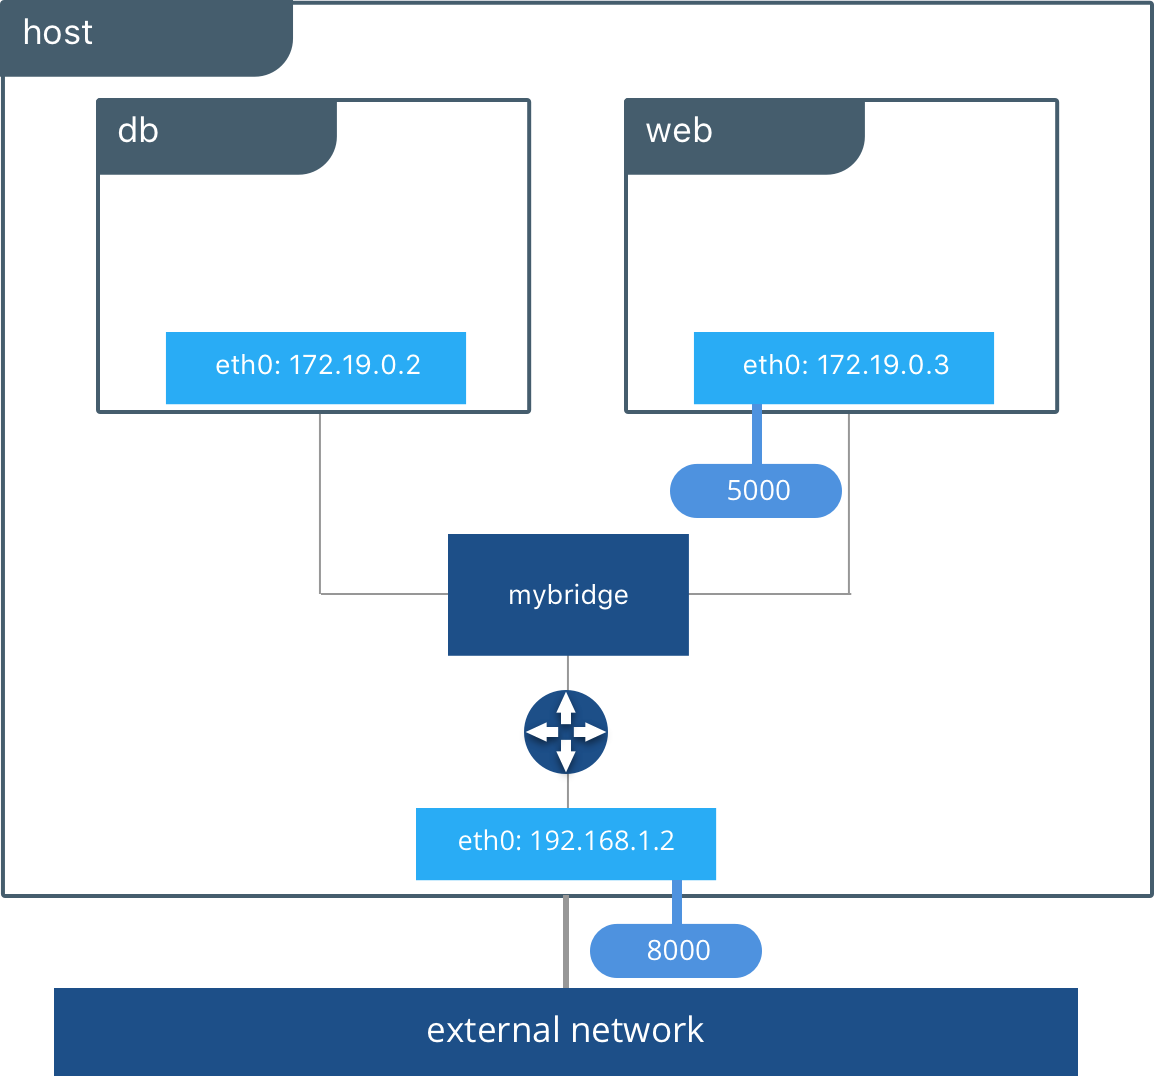
\includegraphics{containernetwork.png}
	}
	\caption{Typical Container Network}
	\caption*{Source:~\cite{dockercontainernetwork}}
\end{figure}

Together, netfilter and Linux's expressive network stack are used to create controllable, highly expressive, and isolated virtual networks for containers.
Virtual interfaces will typically be created for individual containers that are then added to that container's network namespace.
Outside of the container, that interface will often be attached to virtual bridge interfaces, as well as have netfilter, traffic control, and routing rules put in place (e.g.\ NAT on outgoing traffic), to control where to route and how to shape network traffic to or from the container.
This allows for a wide expression of network topologies, has the benefit of being fast to configure with these all being software systems, and allows containers to be relocatable in that they can be moved to other hosts without any disruptions in service availability.
This also ensures that the container can be restricted from viewing the host's actual network, and vice versa where the container can be hidden from the host's network.

% todo: add cites here
This should highlight why container networking is not runtime performant.
Every packet to or from a container must traverse the Linux network stack and netfilter system at least once for every interface, virtual or not, along the container's network path.
For example, if a container has a virtual interface, that is then connected to a virtual bridge, which is then connected to the interface for the NIC\@; that container's network traffic must traverse the Linux network stack a minimum of three times.
With the network stack being primarily implemented in software, meaning both the control plane and data plane are in software, the performance costs explained in Section~\ref{subsec:Networking Planes} can add up.

Putting it together, this, alongside the intra-machine isolation described in Section~\ref{subsec:Containers}, provides an immense amount of power for container deployment.
These systems are extremely quick to configure, highly expressive, and are relatively low overhead\footnote{for most users, other factors like processing time or multiple router hops overshadow the performance cost of container networks, thus container networking is usually considered low overhead}.
Further, container engines are typically used for the actual deployment of containers, such as Docker or podman, that handle the full configuration and monitoring of the aforementioned kernel systems, and use standards for both container images and schemas to describe container deployment.
This makes container deployments simple, consistent across machines, and scalable, which explains why containers have become so widely adopted and why container orchestration tools like Kubernetes have excelled in industry adoption.
As a final note, it is critical to once again emphasize that these are software systems that run inside of the kernel, and thus can only influence operations whose data path cross the kernel.

\subsubsection{RDMA Namespaces and Cgroups}~\label{subsubsec:RDMA Namespaces and Cgroups}
With namespaces and cgroups being the standard systems for isolating Linux kernel resources in containers, there have been developments to add RDMA support for these to the Linux kernel itself.
The \texttt{rdma-system} on Linux integrates with the existing network namespace system to allows for restricting RDMA devices (e.g.\ the \texttt{mlnx4\_0} passed to \texttt{ib\_dev} in most CLIs) from both an \texttt{libibverbs} and \texttt{librdmacm} view to an existing network namespace;
this RDMA device being a physical function, virtual function, or virtualized RDMA NIC (e.g.\ using SoftRoCE).
Further, when an interface (defined by the kernel) for an RDMA device is added to a network namespace, the GID table entries are also added to that namespace, in other words, if a process has a network namespace, it can only see the GID table entries for the interfaces in its network namespace.
% todo: figure out if this is the case for libibverbs too
Next hop resolution is also performed inside of that network namespace~\cite{rdmacmnspatch}.

The RDMA cgroup currently allows for tracking and restricting the number of RDMA control plane resource used (e.g.\ QPs and shared memory regions), and tracking counters exposed by the RDMA device.
Neither of these systems currently integrate with existing kernel network isolation systems like netfilter and do not provide any form of data plane control (e.g.\ restricting the number of work requests), thus on their own, they cannot provide the network virtualization desired for containers.
As such, they currently only provide intra-machine isolation but not inter-machine isolation for RDMA devices~\cite{rdmanamespaceman,rdmacgroups,mellanoxcontainersupdate2018,mlnxcontainerjourney,mlnxrdmadeviceisolation}.


\subsection{Related Work}
\subsubsection{Sharing RDMA NICs Among Virtual Machines}
There's a significant overlap in the research of sharing RDMA NICs among containers and among virtual machines, with many of the to-be-explained solutions being compatible with both.
However, there are some key differences when assessing RDMA NIC sharing for containers:
\begin{enumerate*}[label={(\arabic*)},itemjoin*={{, and }},itemjoin={{, }}]
	\item containers are often ephemeral, thus resource deployment and cleanup must be fast and low overhead
	\item container engines use kernel functionality for isolation, meaning sharing solutions must expose themselves to the kernel in some way
	\item a single machine could run tens to potentially hundreds of containers, as opposed to a handful of virtual machines, thus scalability is more of a concern
	\item containers use a vastly different configuration scheme than virtual machines
\end{enumerate*}.
Due to these differences, solutions like HyV, virtio-RDMA, and vRDMA are incompatible for use in containers and the remaining solutions must be assessed differently for containers than for virtual machines~\cite{fan2017towards,hyvpaper,vrdmavmware}.

\subsubsection{Programmable NICs}
Independent of RDMA, there is a large field of research around programmable NICs (often FPGA based) as a method of speeding up networking.
Network rules, like firewalls, would be programmed into the NIC as a form of hardware offload, as opposed to executing on the CPU through the kernel.
This could be used to express RDMA network rules with minimal performance impact as these rules would run on the NIC itself, therefore allowing for highly-performant container RDMA network isolation.
This too may be part of the future for RDMA device management in containers, but as of now, does not seem mature enough for container use cases or for general use as:
\begin{enumerate*}[label={(\arabic*)},itemjoin*={{, and }},itemjoin={{, }}]
	\item some of these NICs are not available to the public (e.g.\ Azure's programmable NICs)
	\item many of the available programmable NICs are slow or expensive to configure
	\item some NICs exhibit pathological performance characteristics, which is detrimental for RDMA use
	\item these NICs do not integrate with existing kernel network isolation systems (e.g.\ netfilter), thus container engines would have to create complex shim layers to utilize these programmable NICs
\end{enumerate*}~\cite{firestone2018azure,stephens2019loom,katsikas2021you,liu2021performance,kim2020case}.

\subsubsection{eBPF Container Networking}
Many groups have identified netfilter as a massive performance bottleneck for container networking, primarily due to its sequential nature.
Efforts have begun to replace netfilter with eBPF, a system for executing user-space provided code in kernel-space, which would simplify the code paths taken in the kernel for container networking.
While this would alleviate many of the performance impacts of container networking, it would not be a panacea for high performance networking in containers~\cite{ciliumiptablesebpf,ciliumebpf}.
Even with eBPF, container networking would still have to traverse the Linux network stack several times, cross the NIC-CPU boundary for every packet, and cross the user-space/kernel-space boundary to receive and deliver packets;
therefore retaining much of the overhead explained in Section~\ref{subsec:Networking Planes}.
While this may be a solution for those needing faster container networking, RDMA in containers will still be needed for those who want highly performant networking.

\subsubsection{DPDK in Containers}
The Data Plane Development Kit (DPDK) is another, popular form of kernel bypass networking.
Instead of relying on the kernel's networking stack, a user-space process will communicate directly with the NIC and run it's own, custom network stack.
This can be used as a form of high performance networking in containers, but does come with its own unique challenges and research questions.
For example, DPDK often requires heavy CPU utilization, also cannot utilize in-kernel isolation systems, creates more difficulty with network isolation as it has fewer boundaries, and requires privileged containers which may not be desired~\cite{dpdkcontainers,dpdkperformancecontainers,inteldpdk}.
As such, it remains an orthogonal solution to high performance networking in containers.

\section{Overview}
\subsection{Paravirtualized Solutions}
Paravirtualized solutions are those that interpose in some part of the RDMA logic path while keep the rest of the logic path in tact.
Typically, the interposition is done in a part of the logic path that is not hot or performance sensitive (e.g.\ control plane operations) to add additional controllability while maintaining the performance characteristics of RDMA\@.
These solutions tend to require custom libraries, add more code complexity, may require heavier CPU utilization, and require frequent updates to stay in line with the underlying RDMA libraries.
However, they tend to provide close to host-level RDMA performance, tend to scale better than hardware solutions, and can more closely integrate with existing kernel network isolation systems.

% How to test:
% Install Docker
% Configure a Docker macvlan network: `docker network create -d macvlan --subnet=192.168.1.0/24 -o parent=ens3f0 -o macvlan_mode=private mynet`
% Run tests (using rdma_cm to connect, doesn't work without it): docker run --privileged --net=mynet --device=/dev/infiniband --ip 192.168.1.3 -it rdma-mlnx ib_read_bw -d mlx5_0 -R 
%
% Other links:
% https://support.mellanox.com/s/article/docker-roce-macvlan-networking-with-connectx4-connectx5

\subsubsection{Shared HCAs}
Though perhaps not strictly paravirtual given this solution is now built into the RDMA logic path in the kernel, shared HCA operates similarly to paravirtualized solutions in that it interposes namespace and cgroup restrictions in the RDMA control path.
This is arguable the most ``batteries not required'' solution of using RDMA in containers as it uses the built in kernel isolation systems, but is still rudimentary is its expressivity of control.
This solution creates new interfaces (with or without VLAN tags) on top of an RDMA device, then places this interface in the container's network namespace.
As explained in Section~\ref{subsubsec:RDMA Namespaces and Cgroups}, this also places that interface's corresponding GID table entries in the namespace.
Paired with restricting the \texttt{CAP\_NET\_ADMIN} capability for the container, this can then be used to give a container an isolated RDMA interface with a set MAC address, IP address, possible VLAN tag, and restrictions on RDMA resource usage using cgroups.
However, as the RDMA device is not made aware of the host's virtual networks, the interface's properties must be valid on the host's network (e.g.\ the interface must have a valid IP address on the hosts actual network)~\cite{mellanoxdockermacvlan,dockermacvlan}.
This solution is also typically called macvlan mode.

\begin{figure}
	\centering
	\resizebox{0.6\linewidth}{!}{
		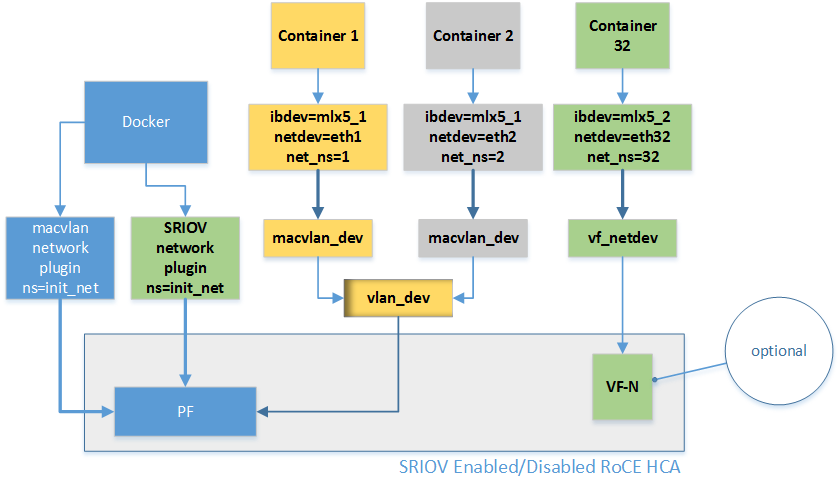
\includegraphics{mlnx_shared_hca_arch.png}
	}
	\caption{Shared HCA Architecture}
	\caption*{Source:~\cite{mellanoxdockermacvlan}}
\end{figure}

\subsubsection*{Container Network Properties}
\begin{description}[nolistsep,font={{\scshape\bfseries}}]
	% todo: fix this part, how does the IP address depend on the NIC?
	\item[Network Isolation] the only isolation provided is the setting of the IP address and VLAN tags on an isolated interface, the IP address is also dependent on the NIC
	\item[Controllability] routing policies and traffic shaping capabilities are not possible unless implemented in the device
	\item[Resource Utilization] aside from GID table entry consumption, resource utilization is identical to normal RDMA usage
\end{description}

\subsubsection*{Performance Tests}
All of the following tests were performed on Cloudlab with two d6515 hosts, which have a 32 core AMD 7452 at 2.35GHz CPU, 128GB RAM, and a dual port ConnectX--5 100 Gbit NIC~\cite{cloudlab}. 
Both were running Ubuntu 20.04 with Linux kernel version 5.4.0, and were using the Mellanox OFED RDMA stack version 5.5-1.0.3.2.

\begin{figure}
	\centering
	\resizebox{0.8\linewidth}{!}{
		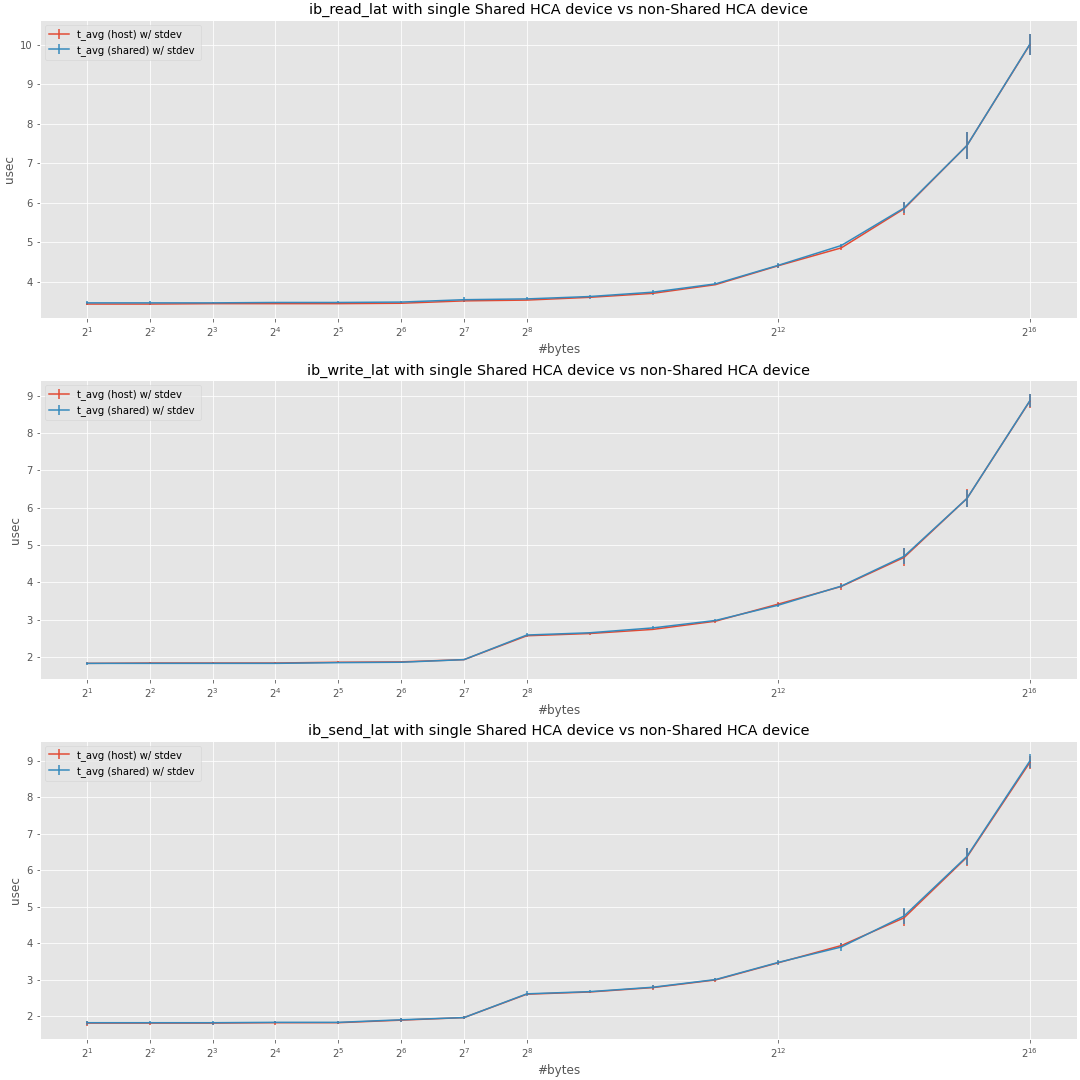
\includegraphics{shared_hca_basic_lat.png}
	}
	\caption{Latency Tests}%
	\label{fig:shared_hca_latency}
\end{figure}

\begin{figure}
	\centering
	\resizebox{0.8\linewidth}{!}{
		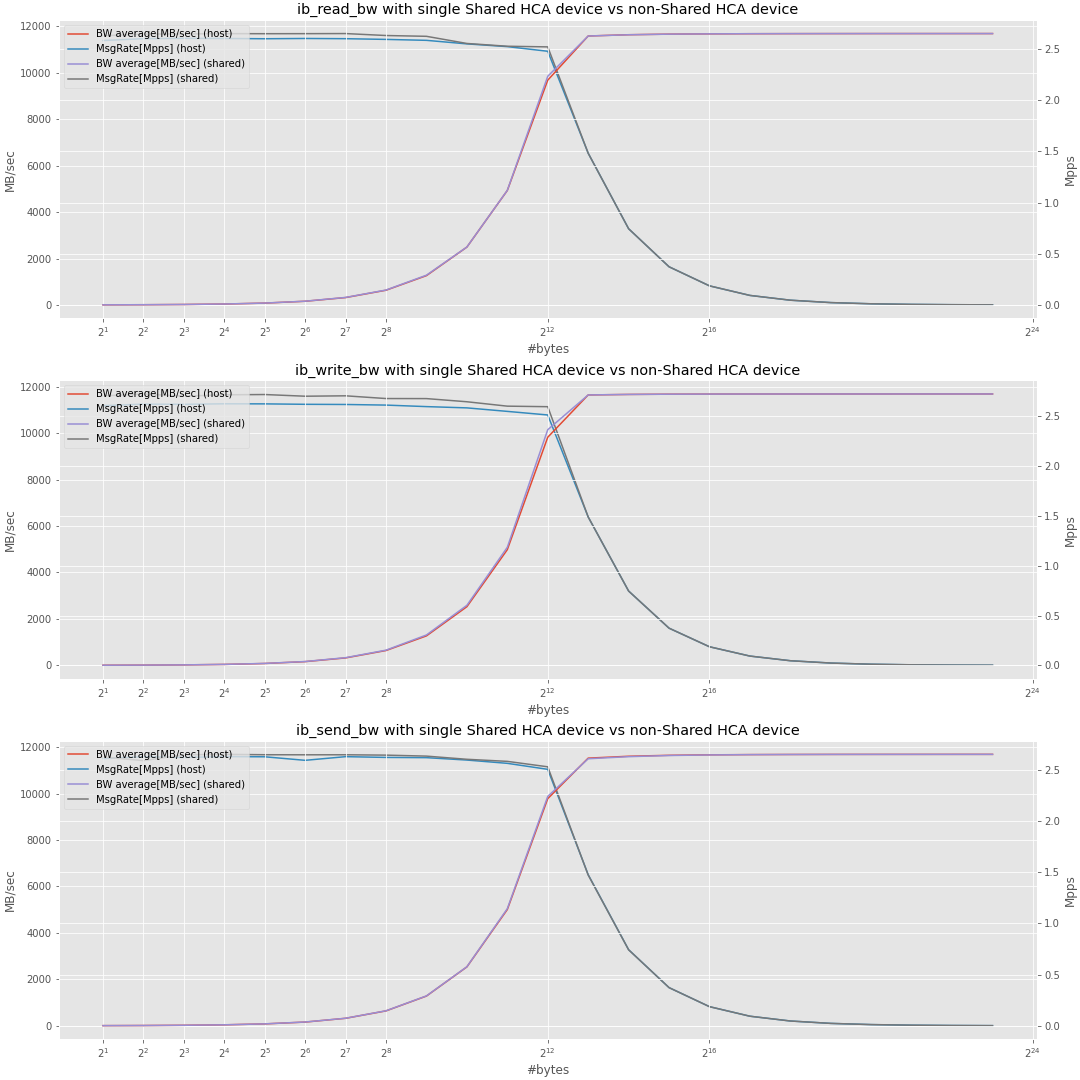
\includegraphics{shared_hca_basic_bw.png}
	}
	\caption{Bandwidth Tests}%
	\label{fig:shared_hca_bandwidth}
\end{figure}

\begin{figure}
	\centering
	\resizebox{0.8\linewidth}{!}{
		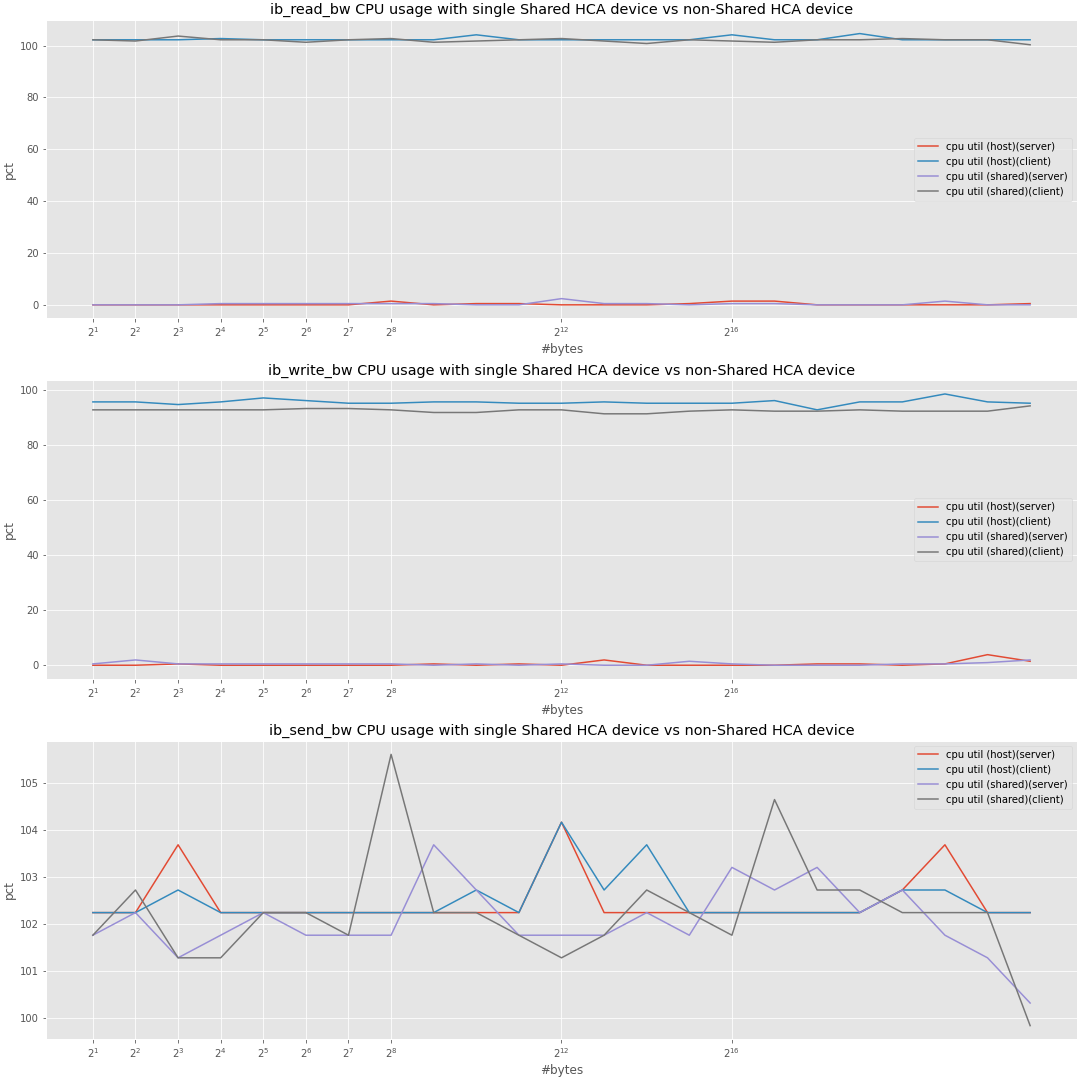
\includegraphics{shared_hca_cpu.png}
	}
	\caption{CPU Utilization}%
	\label{fig:shared_hca_cpu}
\end{figure}

Figures~\ref{fig:shared_hca_latency},~\ref{fig:shared_hca_bandwidth}, and~\ref{fig:shared_hca_cpu} were all performed with either a single shared HCA device (labeled \texttt{shared}) or a single raw RDMA device (labeled \texttt{host}), with varying RDMA message sizes.
All three of these graphs indicate there is no perceivable difference between using the single raw RDMA device vs using a shared HCA device.

\begin{figure}
	\centering
	\resizebox{0.8\linewidth}{!}{
		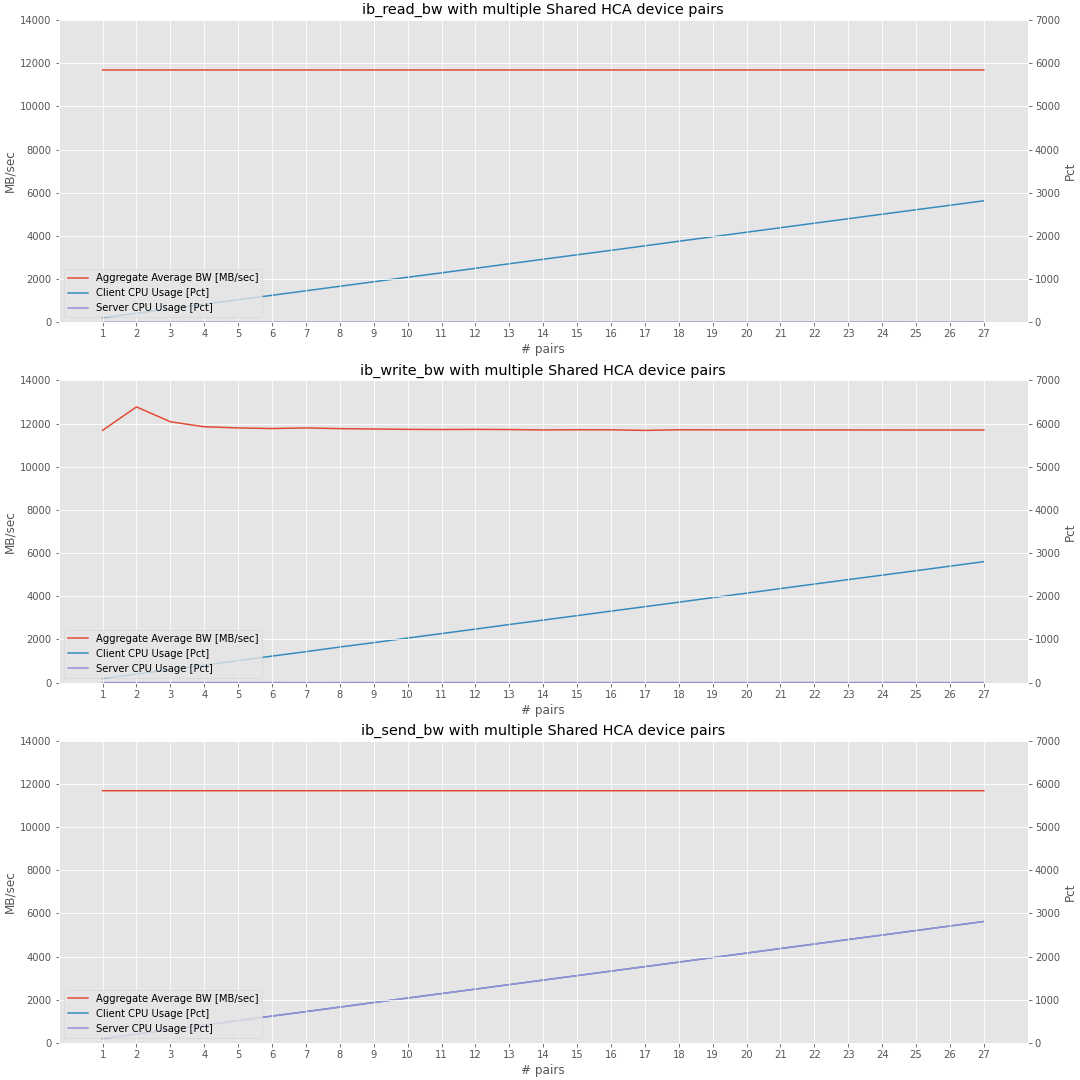
\includegraphics{shared_hca_multi_dev.png}
	}
	\caption{Bandwidth + CPU with Multiple Devices}%
	\label{fig:shared_hca_multi_vdev}
\end{figure}

Figure~\ref{fig:shared_hca_multi_vdev} was performed with multiple shared HCA devices created on both the client and server, with a single \texttt{ib\_(read|write|send)\_bw} test running on each device with a byte size of 65536.
Individual devices on each hosts were connected pair-wise for these tests.
For example, with $\texttt{pairs} = 3$, both the client and server had 3 shared HCA interfaces / devices provisioned.
Shared HCA device 1 on the client connected to the \texttt{ib\_read\_bw} server running on shared HCA device 1 on the server.
Similarly, shared HCA device 2 on the client connected to the \texttt{ib\_read\_bw} server running on shared HCA device 2 on the server, and so on.

Each of these devices were ``provisioned'' by Docker and the tests ran inside of the corresponding Docker container.
Similarly to the individual device tests, the multi-shared HCA device tests show that shared HCA can fully saturate the bandwidth of the host RDMA device with no additional CPU utilization (the CPU utilization is expected with the \texttt{ib\_(read|write|send)\_bw} clients processes using 100\% CPU).
As expected, the use of shared HCA devices requires no performance or resource penalties.

\subsubsection*{Miscellaneous Comments}
\begin{description}[nolistsep,font={{\scshape\bfseries}}]
	\item[Scalability Limits] can only scale to the size of the NIC's GID table, usually below 150 entries
	\item[Proprietary] these features are built into the kernel's RDMA stack thus are available to everyone
	\item[Maturity] have been in development since 2015, so is likely stable enough for use, but is still missing several controllability features; is built into the kernel so likely will be actively maintained
	\item[Ease in Deployment] uses standard kernel isolation systems, thus is similar in ease of deployment as containers
	\item[Execution Privileges] requires no additional privileges
	\item[Network Pressure] requires a unique IP address per interface, thus can result in IP address exhaustion or network switch table exhaustion
\end{description}

For those that don't need virtual network control for RDMA, do not anticipate running hundreds of RDMA containers, and do not require fine grain traffic shaping of RDMA packets (or are fine relying on the network or global NIC policies for it), this would be an excellent solution.
However, unless unique IP addresses for containers are required (e.g.\ for network level routing policies), it is likely more beneficial to directly expose RDMA devices to containers.

% TODO: add a section on Freeflow's design flaws around rkey mapping
% specifically, RDMA frequently has duplicate rkeys (see https://www.usenix.org/system/files/sec21_slides_rothenberger_0.pdf)
% this breaks Freeflow's rkey mapping scheme in its entirety.
\subsubsection{FreeFlow}
FreeFlow operates in a far more paravirtualized style with the use of a user-space library and controller interposing in the RDMA control paths.
It claims to provide close to bare-metal RDMA performance, while adding significantly more controllability to RDMA operations, thereby allow for performant use inside of containers.
It does this with two key features:
\begin{enumerate*}[label={(\arabic*)},itemjoin*={{, and }},itemjoin={{, }}]
	\item communications to RDMA character devices (i.e.\ \texttt{uverbs0}) and consumption of work requests is instead routed to and processed by a controller (FreeFlow Router)
	\item the data path for \textit{payloads} are kept in-tact using shared memory
\end{enumerate*};
these being implemented in two pieces of software: the FreeFlow Library (FFL) and FreeFlow Router (FFR).

Breaking this down, containers that use RDMA devices must use a modified form of the \texttt{libibverbs} library called the FreeFlow Library.
This library forwards all \texttt{libibverbs} operations through an IPC channel, instead of the normal RDMA character devices, to a running FreeFlow Router process.
This results in all of the RDMA control plane and most of the data plane flowing through FreeFlow, with the most critical parts of the data plane being kept intact.
This is implemented as the following:
\begin{enumerate}[nolistsep]
	\item The FFR maintains virtual RDMA device information per container, for which it returns information about to the container when the container uses \texttt{libibverbs} operations like \texttt{ibv\_query\_device}.
	\item The FFR maintains the true RDMA queue pairs for those virtual RDMA devices. This allows it to rewrite addressing information (such as dgid) when the container creates new queue-pairs.
	\item On shared memory registration, the container (through the FFL) will shared those memory regions with the FFR, which then shares it with the NIC\@. Recall this shared memory region is where the RDMA message payloads live, thus this allows for one-sided and two-sided RDMA operations and keeps the hottest part of the RDMA data path in tact.
	\item A container will post work requests through the IPC channel, which the FFR then processes and can apply traffic shaping rules to. Alternatively, the container can create ``fake'' queue-pairs in a region of memory shared with the FFR, on which the FFR will spin-loop on. When it reads a new work request, the FFR will process it with traffic shaping rules and copy it to the true queue pairs. This alternative mode, called FastPath, allows for lower latency, but requires the use of an entire CPU core.
\end{enumerate}
This clever interposition in the least performance critical parts of RDMA allow for significantly more isolation and controllability, and allows for integrations with existing network isolation systems~\cite{kim2019freeflow}.

\begin{figure}
	\centering
	\resizebox{0.6\linewidth}{!}{
		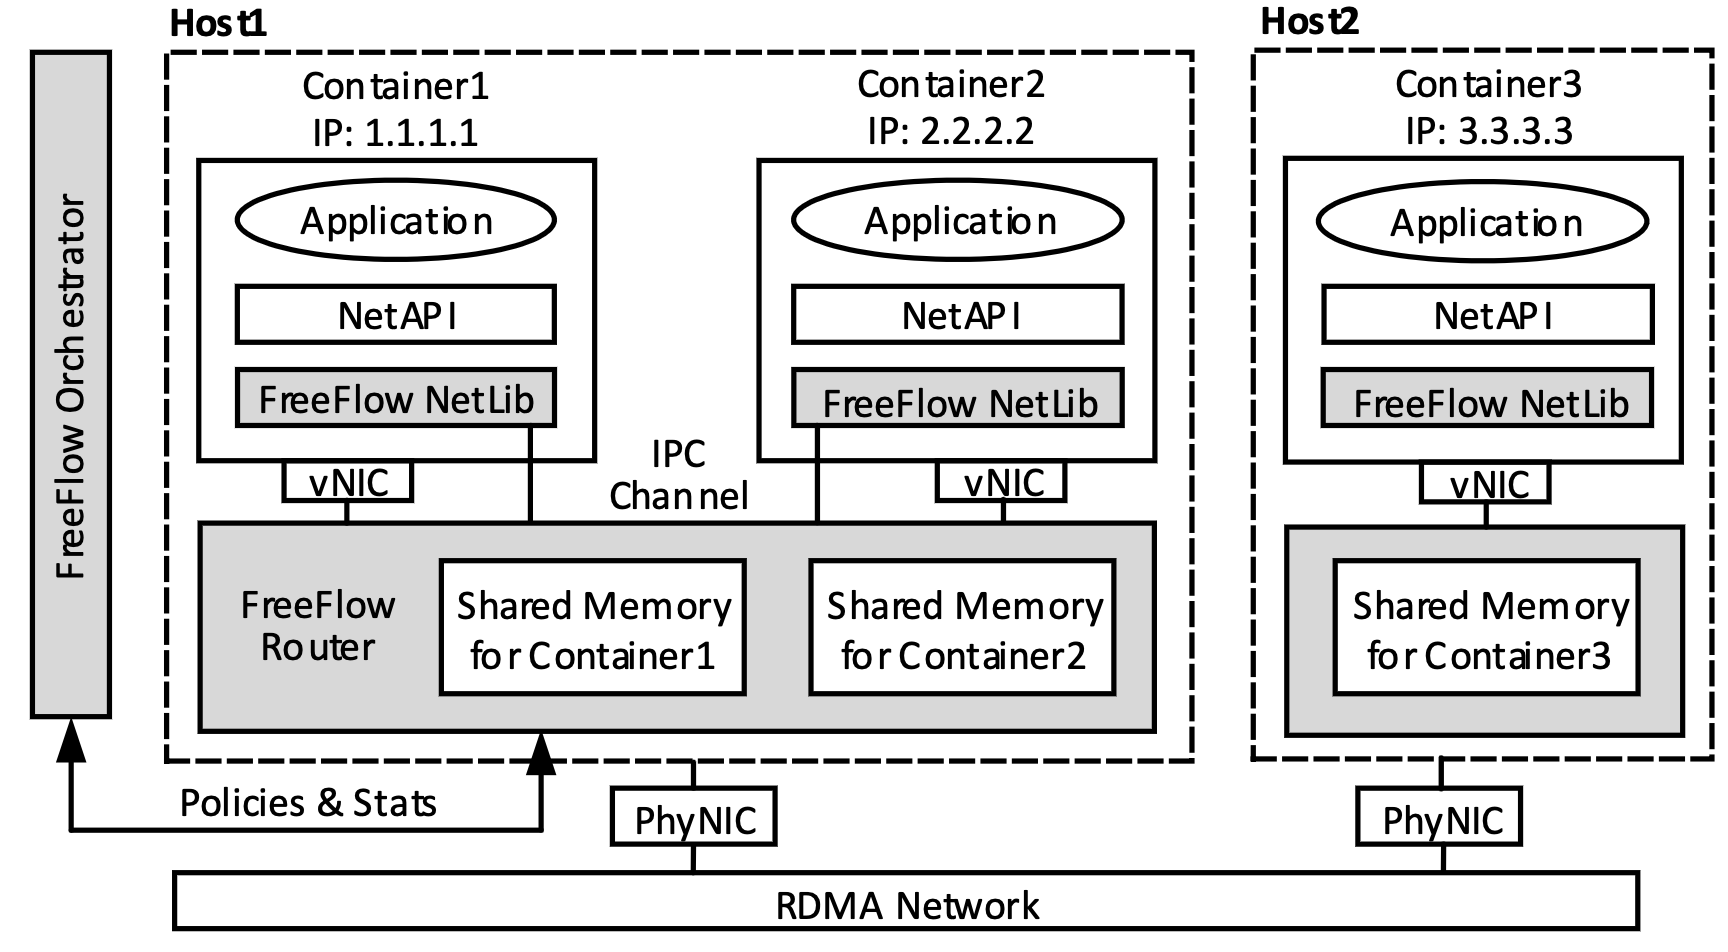
\includegraphics{freeflow_arch.png}
	}
	\caption{FreeFlow Architecture}
	\caption*{Source:~\cite{kim2019freeflow}}
\end{figure}

\subsubsection*{Container Network Properties}
\begin{description}[nolistsep,font={{\scshape\bfseries}}]
	\item[Network Isolation] each container is given its own virtual RDMA device, ``namespace'' in the FreeFlow Router, and is not exposed to the NIC's actual network, thus allowing for the same level of isolation as standard container networks
	\item[Controllability] allows for full control over the routing and traffic shaping of RDMA messages
	\item[Resource Utilization] can require the use of an entire CPU core (or more) for low latency needs, otherwise uses no more overhead than one additional running process
\end{description}

\subsubsection*{Performance Tests}
All of the following tests were performed on Cloudlab with two c6220 hosts, which have a 2, 8 core Intel Xeon E5-2650v2 at 2.6GHz CPUs, 64GB RAM, and a single port ConnectX--2 FDR (40 Gbit) Infiniband NIC~\cite{cloudlab}. 
Both were running Ubuntu 20.04 with Linux kernel version 5.4.0, and were using the Mellanox OFED RDMA stack version 4.9-4.1.7.0.
The Freeflow stack used is a fork (developed for this thesis) of the official Microsoft Freeflow repository, having been updating from the MLNX OFED 4.0 stack to the 4.9 stack.
This fork also includes a handful of patches to fix Freeflow's rkey mappings and the build process.

Freeflow provides two modes.
The first, fastpath, polls for completed work requests on the client side to provide improved latency results at the cost of a fully pinned CPU core.
The second, no fastpath, waits for messages from the unix socket shared with the Freeflow router, which reduces CPU utilization but increases latency.
Both are tested and their results are reported here. 
Unfortunately, it appears no fastpath suffers from deadlocks with specific RDMA message sizes and with multiple Freeflow clients, thus its results are more limited than the fastpath version.

\begin{figure}
	\centering
	\resizebox{0.8\linewidth}{!}{
		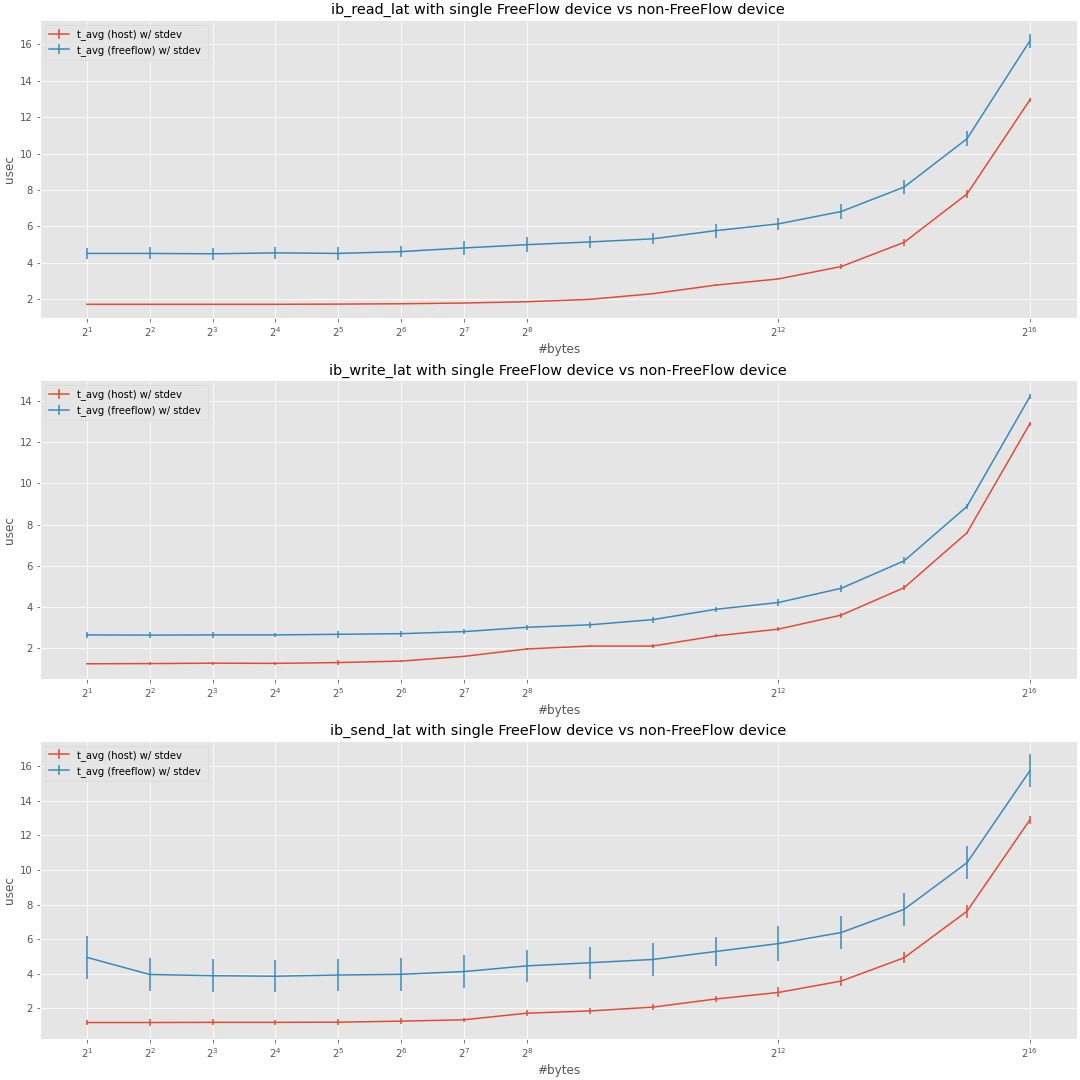
\includegraphics{freeflow_basic_lat.png}
	}
	\caption{Fastpath Latency Tests}%
	\label{fig:freeflow_latency}
\end{figure}

\begin{figure}
	\centering
	\resizebox{0.8\linewidth}{!}{
		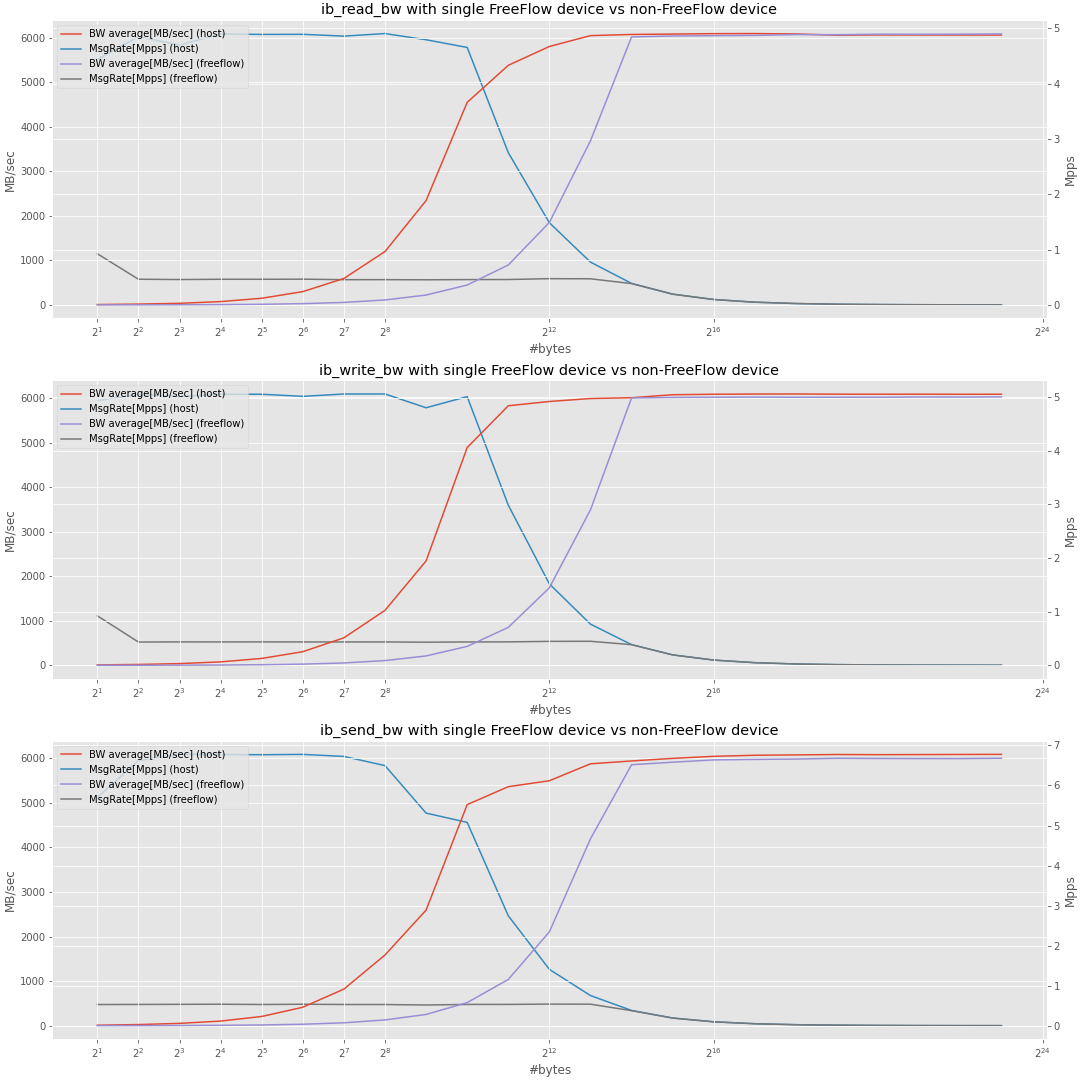
\includegraphics{freeflow_basic_bw.png}
	}
	\caption{Fastpath Bandwidth Tests}%
	\label{fig:freeflow_bandwidth}
\end{figure}

\begin{figure}
	\centering
	\resizebox{0.8\linewidth}{!}{
		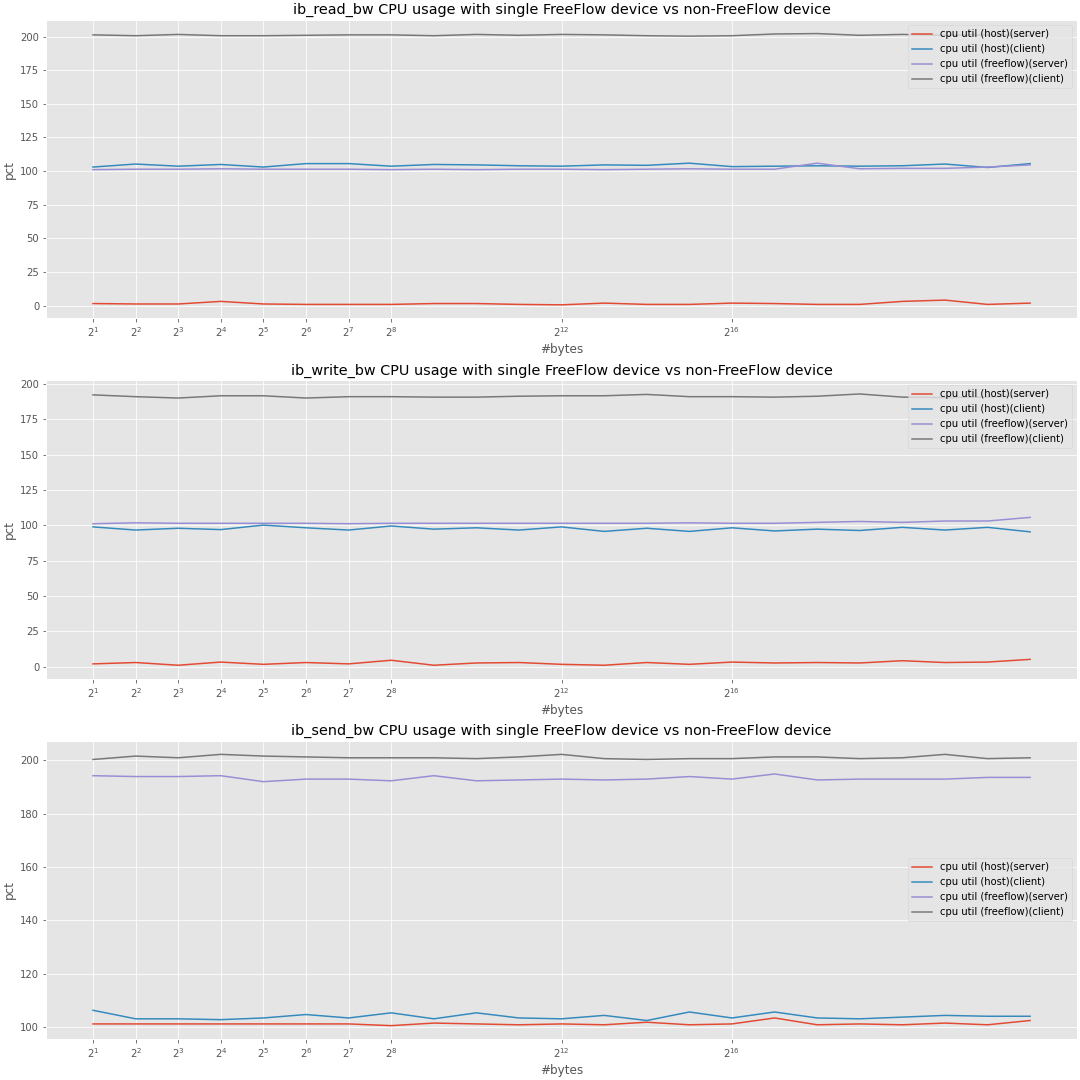
\includegraphics{freeflow_cpu.png}
	}
	\caption{Fastpath CPU Utilization}%
	\label{fig:freeflow_cpu}
\end{figure}

Figures~\ref{fig:freeflow_latency},~\ref{fig:freeflow_bandwidth}, and~\ref{fig:freeflow_cpu} were all performed with either a single Freeflow device (labeled \texttt{freeflow}) or a single raw RDMA device (labeled \texttt{host}), with varying RDMA message sizes.
Figure~\ref{fig:freeflow_latency} indicates that, even with the client and Freeflow router spinning on the completion queue, there is still a significant latency overhead to using Freeflow.
Figure~\ref{fig:freeflow_bandwidth} shows that Freeflow is capable of fully saturating the NIC's bandwidth, albeit requiring almost 4 times the RDMA message sizes than when using the raw host RDMA device.
This appears to be from Freeflow's inability to handle large message rates, which lags considerable behind the message rate achievable when using the raw host RDMA device.
As this is primarily a CPU bound limitation, Freeflow may see significantly better bandwidth performance on higher clock rate CPUs.
Figure~\ref{fig:freeflow_cpu} shows Freeflow using double the CPU on both the server and client when compared to using the raw host RDMA device.
This is likely due to the use of fastpath, which pins the Freeflow router at 100\% CPU utilization on both the client and server. 
Aside from this, Freeflow doesn't appear to require any additional CPU utilization.

\begin{figure}
	\centering
	\resizebox{0.8\linewidth}{!}{
		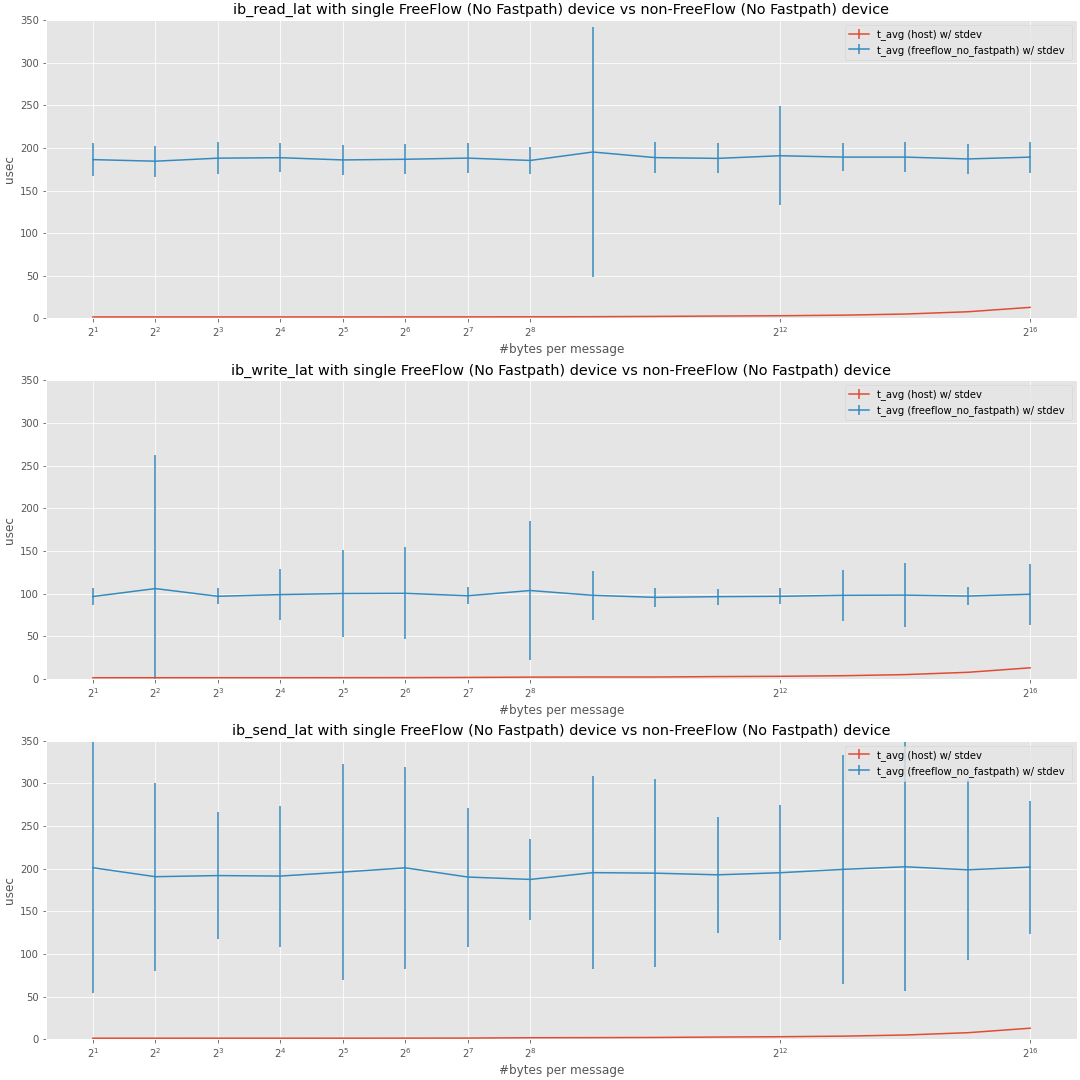
\includegraphics{freeflow_no_fastpath_basic_lat.png}
	}
	\caption{No Fastpath Latency Tests}%
	\label{fig:freeflow_no_fastpath_latency}
\end{figure}

\begin{figure}
	\centering
	\resizebox{0.8\linewidth}{!}{
		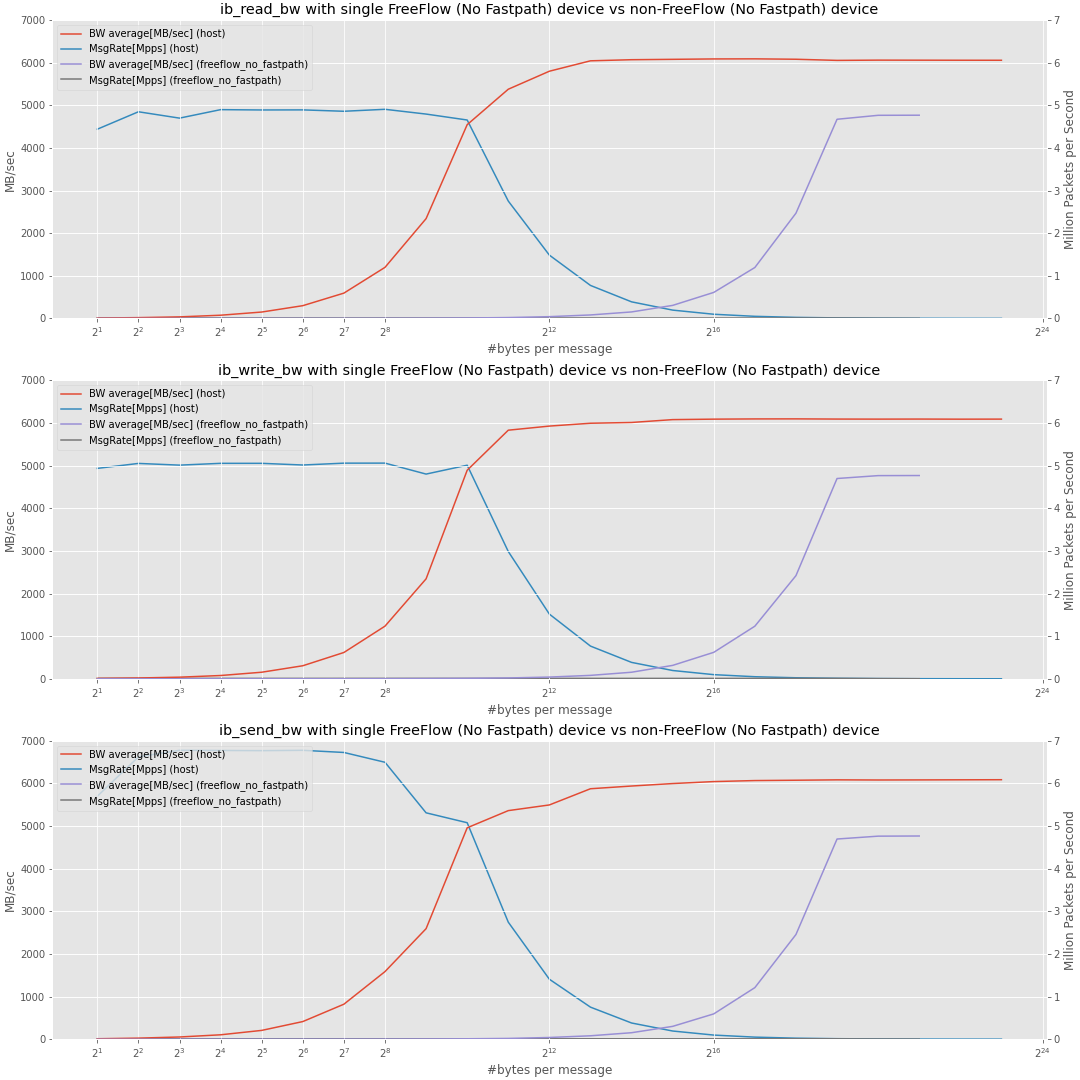
\includegraphics{freeflow_no_fastpath_basic_bw.png}
	}
	\caption{No Fastpath Bandwidth Tests}%
	\label{fig:freeflow_no_fastpath_bandwidth}
\end{figure}

\begin{figure}
	\centering
	\resizebox{0.8\linewidth}{!}{
		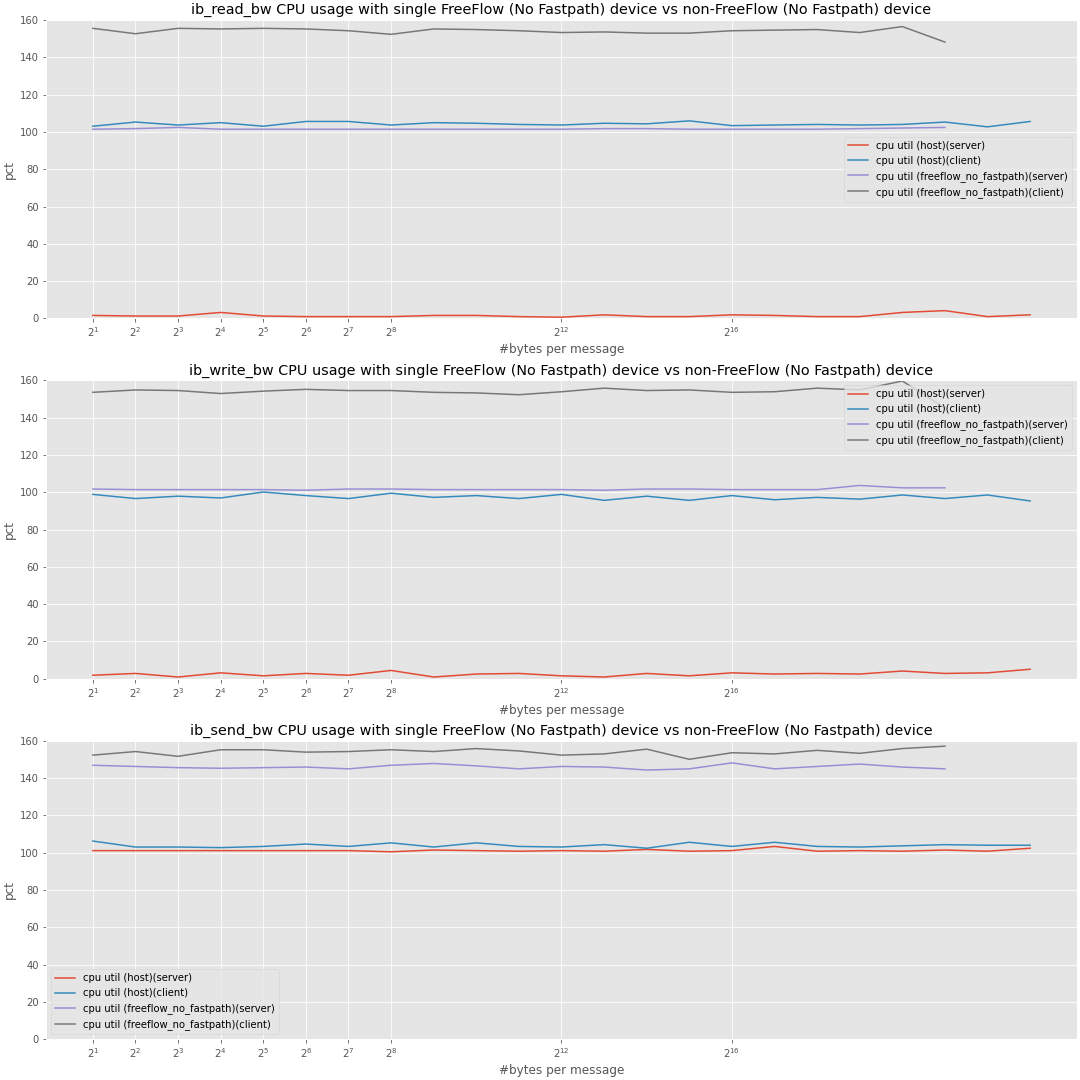
\includegraphics{freeflow_no_fastpath_cpu.png}
	}
	\caption{No Fastpath CPU Utilization}%
	\label{fig:freeflow_no_fastpath_cpu}
\end{figure}

Figures~\ref{fig:freeflow_no_fastpath_latency},~\ref{fig:freeflow_no_fastpath_bandwidth}, and~\ref{fig:freeflow_no_fastpath_cpu} were all performed with either a single Freeflow device in non-fastpath mode (labeled \texttt{freeflow}) or a single raw RDMA device (labeled \texttt{host}), with varying RDMA message sizes.
Figure~\ref{fig:freeflow_no_fastpath_latency} shows a extreme increase in the latency overhead when compared to using Freeflow with fastpath.
This confirms, as mentioned in the paper, that non-fastpath mode is unacceptable for any latency sensitive purposes.
Figure~\ref{fig:freeflow_no_fastpath_bandwidth} indicates that non-fastpath mode also suffers substantially in bandwidth; 
it is no longer capable of fully saturing the NIC's bandwidth like Freeflow with fastpath was able to.
This is likely due to the even worse message rate handling with the non-fastpath mode, as the message rate is bottle necked by the notifications sent from the Freeflow router to the Freeflow client through the unix socket.
Data past 2097152 bytes is not reported for Freeflow without fastpath as the Freeflow router appears to locks up after this message size.

\begin{figure}
	\centering
	\resizebox{0.8\linewidth}{!}{
		\includegraphics{freeflow_multi_vdev.png}
	}
	\caption{Bandwidth + CPU with Multiple Devices}%
	\label{fig:softroce_multi_vdev}
\end{figure}

\subsubsection*{Miscellaneous Comments}
\begin{description}[nolistsep,font={{\scshape\bfseries}}]
	\item[Scalability Limits] can feasibly scale to hundreds of containers as it is constrained only by the available hardware on the host, not the NIC
	\item[Proprietary] FreeFlow is available to use on GitHub and uses the standard \texttt{libibverbs} library
	\item[Maturity] has not been maintained since publication and relies on an older \texttt{libibverbs} version, thus is not mature enough for general use
	\item[Ease in Deployment] it does not currently plug into existing container orchestration tools and requires patching headers for us, thus is not easy to deploy
	\item[Execution Privileges] requires the FreeFlow Router to be a privileged container (if it runs in one), but client containers do not have to be privileged
	\item[Network Pressure] virtual FreeFlow RDMA devices are not exposed to the network, thus creates no additional network pressure
\end{description}

While FreeFlow seems like a promising solution and does not rely on the RDMA hardware capabilities, it suffers from being an unmaintained research project and is, unfortunately, not fit for general use.
Further, FreeFlow, even with FastPath enabled, exhibits latency penalties on small message sizes, thus is likely not viable for latency sensitive applications.

\subsubsection{MasQ}
MasQ operates almost identically to FreeFlow, but instead leaves the entire RDMA data plane intact.
This meaning that queue pairs live in the container's memory space and are directly exposed to the RDMA device, thereby allowing for low latency RDMA operations without the need for a pinned CPU core like FreeFlow.
This comes at the cost of being unable to enforce traffic shaping policies, as the controller is no longer on the RDMA data plane.
However, as the controller is still interposed in the RDMA control plane, address translation, routing policies, and the notion of virtual RDMA devices is still applicable.

MasQ is not publicly available and is similar enough to FreeFlow that it will not be fully elaborated on.
The key differences between MasQ and FreeFlow are:
\begin{enumerate*}[label={(\arabic*)},itemjoin*={{, and }},itemjoin={{, }}]
	\item reduced controllability
	\item reduced resource utilization
	\item improved latency performance
\end{enumerate*};
as well as being proprietary and inaccessible for public use~\cite{he2020masq}.

\subsection{Hardware Solutions}
Hardware solutions rely on functionality built into the RDMA-capable NIC itself.
While these solutions tend to be the fastest as they require no software interposition from the kernel, they tend to be highly proprietary and costly, require the newest versions of RDMA-capable NICs, and are often not compatible with older RDMA-capable NICs.
Further, they to have strict scalability limits as hardware resources on NICs are limited.

% References:
% https://support.mellanox.com/s/article/howto-configure-sr-iov-for-connect-ib-connectx-4-with-kvm--infiniband-x
% https://docs.nvidia.com/networking/pages/viewpage.action?pageId=52014524#SingleRootIOVirtualization(SRIOV)-settingupsr-iovSettingUpSR-IOV

\subsubsection{SR-IOV}
As explained in Section~\ref{subsubsec:Control Plane}, SR-IOV is a method of multiplexing RDMA-capable NICs in hardware and is traditionally used in the context of virtual machines.
It has seen adoption as an RDMA in container solution as each virtual function of an RDMA-capable NIC is exposed as a unique, isolated RDMA device that can then be used by individual containers.
These virtual functions can then be plugged into RDMA namespaces to isolate each container's RDMA view to just that singular RDMA device.
Further, with SR-IOV being a hardware feature, some RDMA-capable NICs allow for hardware enforcement of VLAN tagging and flow control per virtual function, which could then be applied to SR-IOV usage in containers.

Recall that SR-IOV cannot scale past a certain number of virtual functions due to hardware resource limitations.
Further, because these are still hardware devices, virtual functions cannot integrate with kernel network isolation systems.

\subsubsection*{Container Network Properties}
\begin{description}[nolistsep,font={{\scshape\bfseries}}]
	% todo: fix this part, how does the IP address depend on the NIC?
	\item[Network Isolation] each NIC is given its own RDMA device, which can have its own IP address and VLAN tags; however the IP address must be exposed to the host network
	\item[Controllability] routing policies and traffic shaping capabilities are not possible unless implemented in the device
	\item[Resource Utilization] consumes SR-IOV slots in the NIC and can exhaust the GID table of the NIC, however does not require any other resources
\end{description}

\subsubsection*{Performance Tests}
All of the following tests were performed on Cloudlab with two d6515 hosts, which have a 32 core AMD 7452 at 2.35GHz CPU, 128GB RAM, and a dual port ConnectX--5 100 Gbit NIC~\cite{cloudlab}. 
Both were running Ubuntu 20.04 with Linux kernel version 5.4.0, and were using the Mellanox OFED RDMA stack version 5.5-1.0.3.2.

\begin{figure}
	\centering
	\resizebox{0.8\linewidth}{!}{
		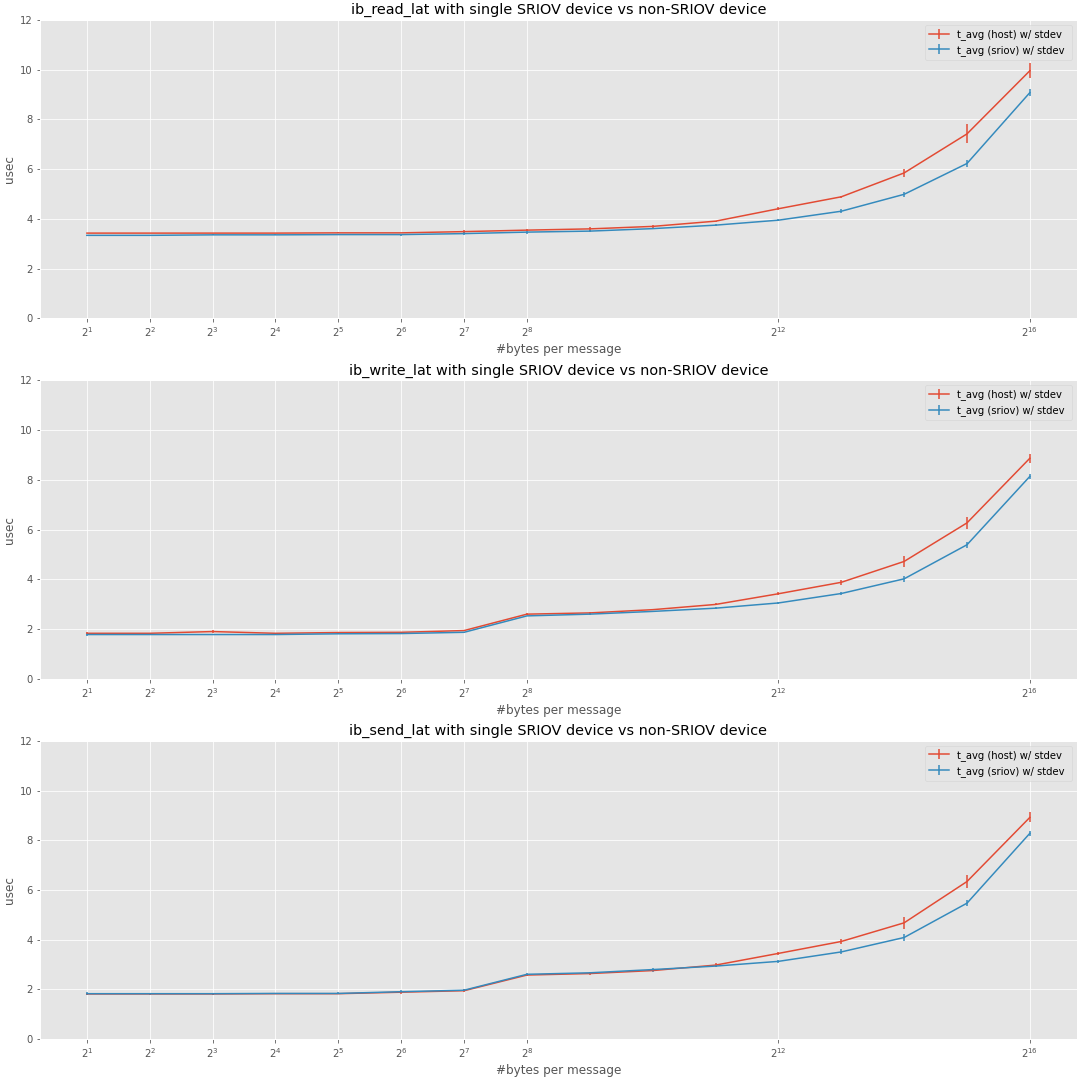
\includegraphics{sriov_basic_lat.png}
	}
	\caption{Latency Tests}%
	\label{fig:sriov_latency}
\end{figure}

\begin{figure}
	\centering
	\resizebox{0.8\linewidth}{!}{
		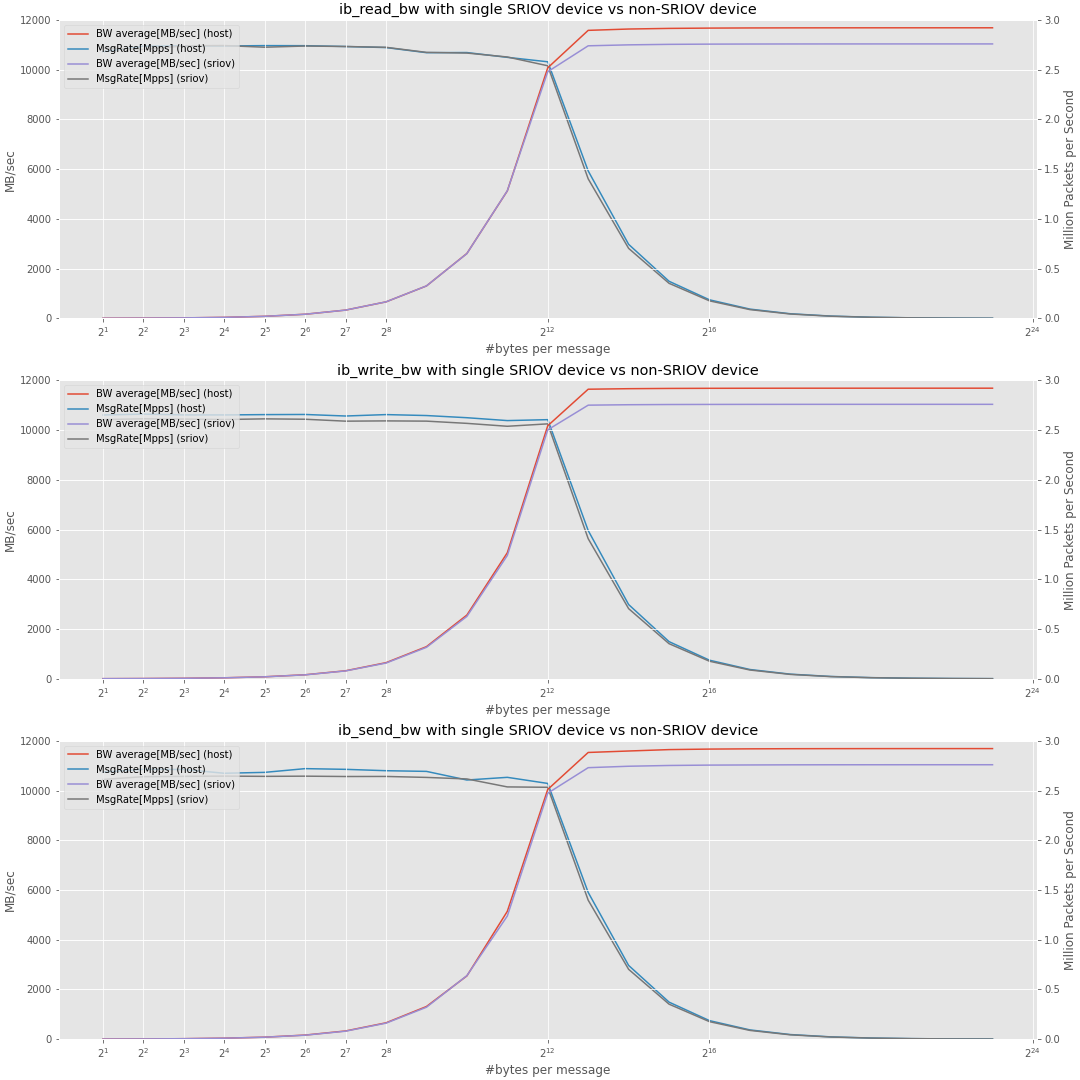
\includegraphics{sriov_basic_bw.png}
	}
	\caption{Bandwidth Tests}%
	\label{fig:sriov_bandwidth}
\end{figure}

\begin{figure}
	\centering
	\resizebox{0.8\linewidth}{!}{
		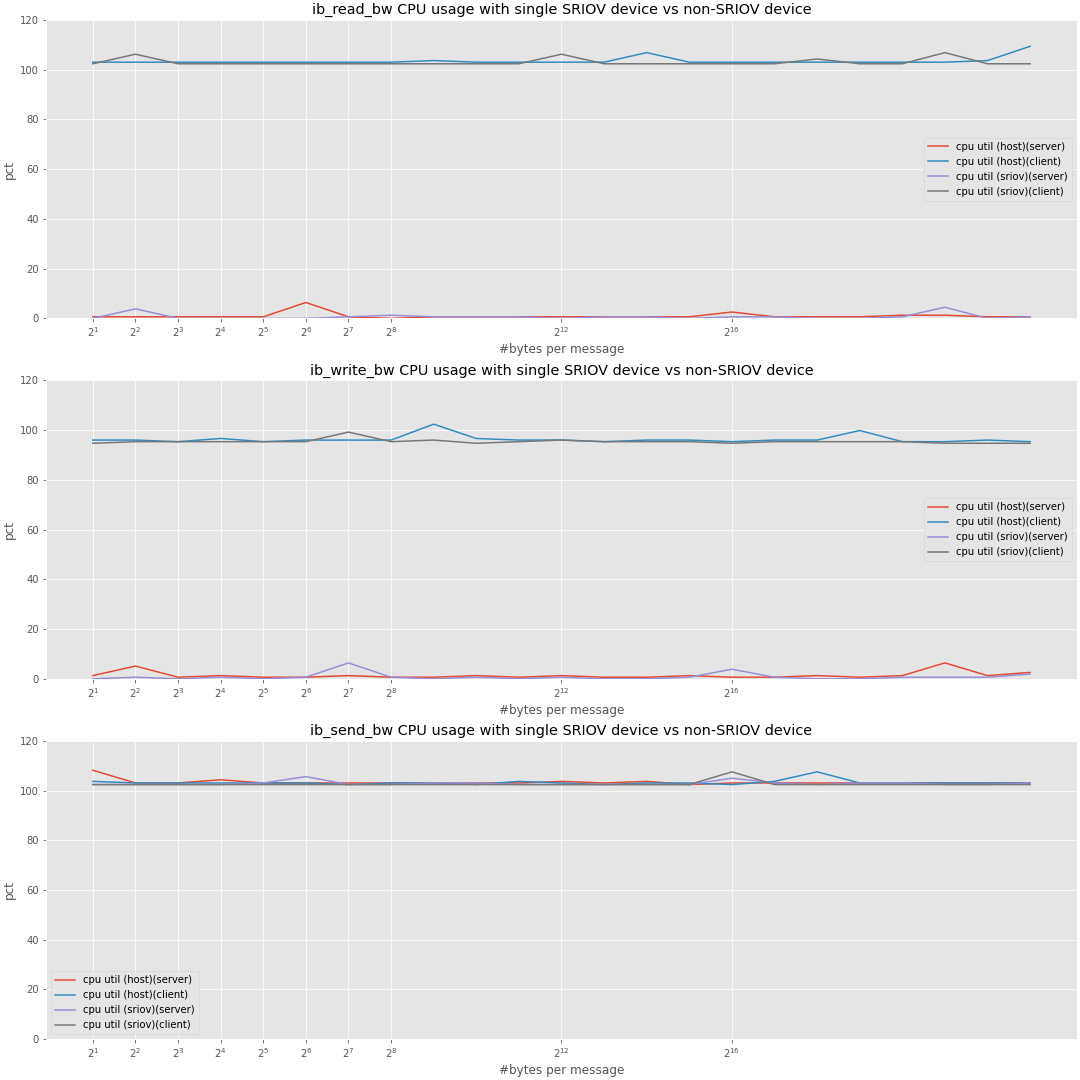
\includegraphics{sriov_cpu.png}
	}
	\caption{CPU Utilization}%
	\label{fig:sriov_cpu}
\end{figure}

Figures~\ref{fig:sriov_latency},~\ref{fig:sriov_bandwidth}, and~\ref{fig:sriov_cpu} were all performed with either a single SR-IOV device (labeled \texttt{sriov}) or a single raw RDMA device (labeled \texttt{host}), with varying RDMA message sizes.
The use of SR-IOV does appear to have a small, but significant network performance impact.
Figure~\ref{fig:sriov_latency} shows that latency appears to be slightly worse for small message sizes and becomes up to 1 microsecond worse with larger payloads.
Figure~\ref{fig:sriov_bandwidth} shows that, for bandwidth, SR-IOV appears to be capped at about 500 to 1000 MB/sec less than if using the raw host RDMA device.
As expected, Figure~\ref{fig:sriov_cpu} shows CPU performance is not worse when using an SR-IOV device as all of the device multiplexing is done on the NIC itself. 

\begin{figure}
	\centering
	\resizebox{0.8\linewidth}{!}{
		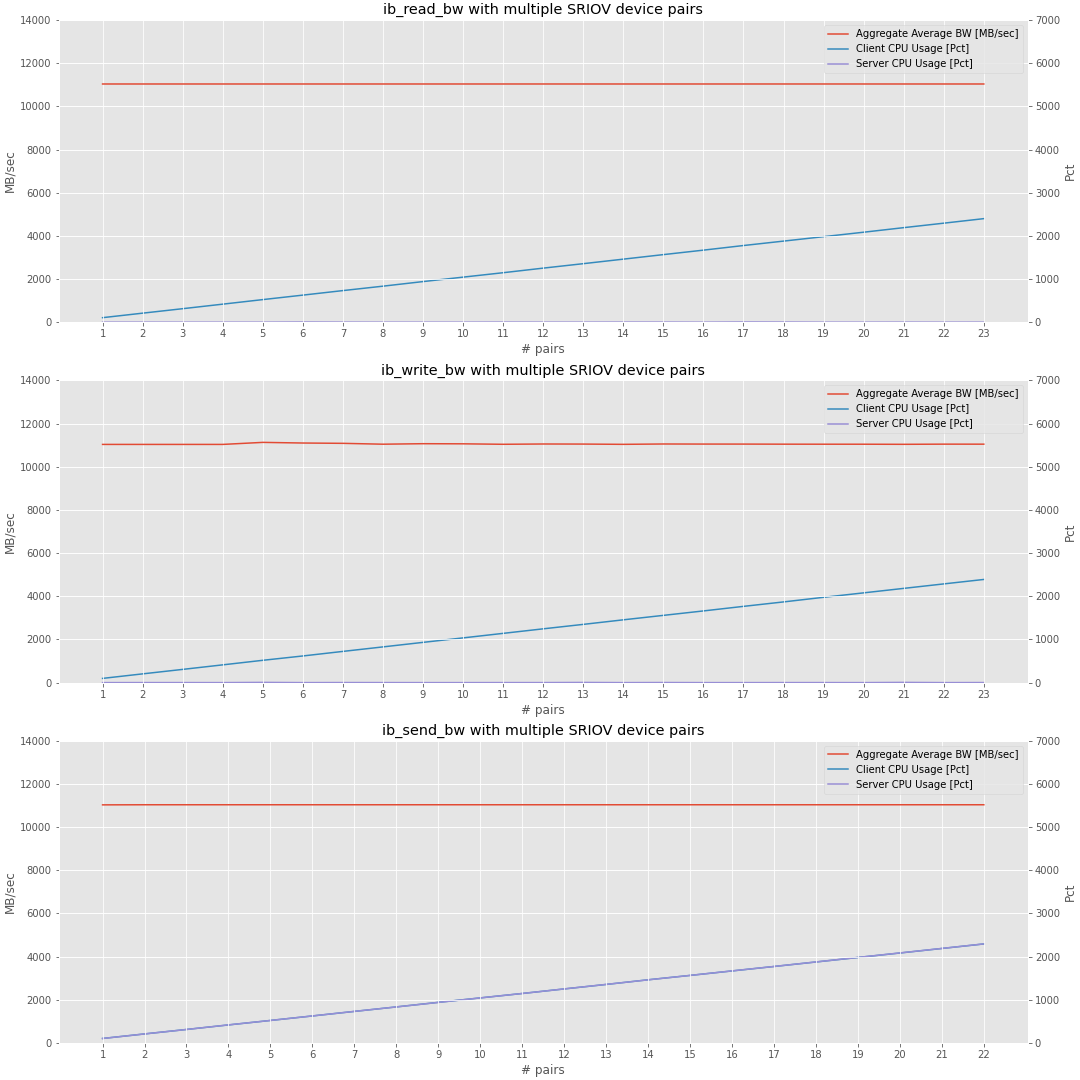
\includegraphics{sriov_multi_dev.png}
	}
	\caption{Bandwidth + CPU with Multiple Device}%
	\label{fig:sriov_multi_vdev}
\end{figure}

Figure~\ref{fig:sriov_multi_vdev} was performed with multiple SR-IOV devices created on both the client and server, with a single \texttt{ib\_(read|write|send)\_bw} test running on each device with a byte size of 65536.
SR-IOV appears to not suffer in bandwidth with the use of additional SR-IOV devices, indicating its performance scales nicely.
However, similar to the single device tests, it seems that even the use of multiple SR-IOV devices has a bandwidth cap less than what is achievable with the raw host RDMA device.

\subsubsection*{Miscellaneous Comments}
\begin{description}[nolistsep,font={{\scshape\bfseries}}]
	\item[Scalability Limits] limited by both the number of possible SR-IOV virtual functions on the NIC, as well as the number of GID table entries available (ex.\ for RoCEv2, SR-IOV VFs need at least 2 entries)
	\item[Proprietary] requires the NIC hardware to support it, some controllability features like flow control are dependent on the NIC features as well
	\item[Maturity] has been commonly used for virtual machines and is mature enough for general use
	\item[Ease in Deployment] requires custom handlers for container engines to provision, but these are commonly provided by NIC vendors thus is relatively easy to deploy
	\item[Execution Privileges] requires privileges to provision (and possibly control) new SR-IOV NICs
	\item[Network Pressure] requires new IP address and MAC addresses for each virtual function on Ethernet; adds no additional network pressure on Infiniband
\end{description}

SR-IOV provides many of the same benefits as shared HCA, thus in most situations, it may be advisable to use shared HCAs instead to avoid the limit on the number of possible virtual functions and the slight performance penalty for using SR-IOV\@.
However, shared HCAs do not fully isolate RDMA devices and do not integrate as nicely with the control features of the NIC hardware, thus if this these are required, SR-IOV may be more desirable~\cite{mlnxofedmanual,mellanoxdockersriov}.

\subsubsection{Hardware Offload: Mellanox's ASAP$^2$ Direct}
% TODO: does this plug in with shared HCA? can this do port mapping to allow multiple RDMA ports?
Hardware offload allows for executing certain routing and traffic shaping policies on the NIC's hardware --- potentially with specialized hardware like FPGAs --- instead of in the kernel.
This provides significant performance gains in the execution of networking policies, and can potentially result in elimination of CPU interposition in network policy enforcement all together.
However, most forms of hardware offload have been limited in their expressiveness, for example being limited to very specific TCP offloads, thus were not capable of executing the complex policies required for container networks.
This has changed with modern NICs, particularly high performance NICs like those supporting RDMA operations, which have added hardware offload support for software defined network policies (e.g.\ Open-vSwitch policies).
If these policies are expressive enough they can be used for container isolation and, subsequently, inter-machine RDMA isolation with minimal overhead and with negligible performance impact.

One notable and more accessible hardware offload system that supports RDMA is Mellanox's ASAP$^2$ Direct, which allows for executing Open-vSwitch policies and operations on the NIC hardware~\cite{mellanoxdockerovs}.
Together with SR-IOV, ASAP$^2$ Direct can be used for full hardware enforced inter and intra-machine RDMA device isolation;
allowing for extremely performant, isolated use of RDMA inside of containers.
ASAP$^2$ Direct is not the only form of hardware offload for RDMA, but may be the most accessible given the prevalence of ConnectX series NICs in high performance computing environments and with it not being a cloud proprietary solution (e.g.\ Azure accelerated NICs).
Thus, while these characteristics are not necessarily generalizable to all hardware offloads systems, it's characteristics will be described below to give a general overview of what one form of hardware offload can provide.

\begin{figure}
	\centering
	\resizebox{0.6\linewidth}{!}{
		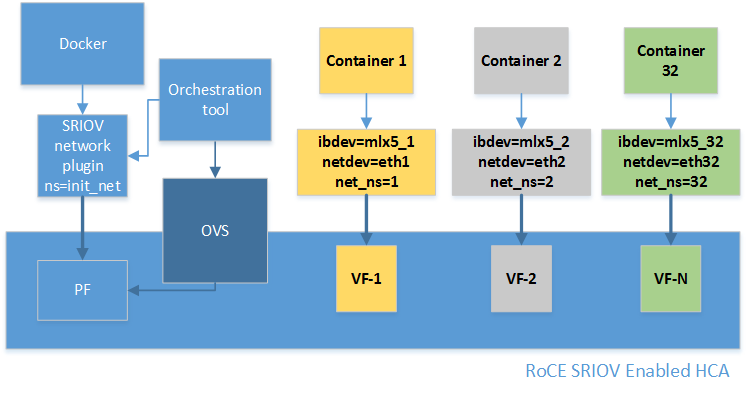
\includegraphics{mlnx_sriov_ovs_arch.png}
	}
	\caption{SR-IOV + OVS (w/ ASAP$^2$ Direct Hardware Offload) Architecture}
	\caption*{Source:~\cite{mellanoxdockerovs}}
\end{figure}

\subsubsection*{Container Network Properties}
\begin{description}[nolistsep,font={{\scshape\bfseries}}]
	\item[Network Isolation] when used with SR-IOV, full network isolation can be achieved, otherwise hardware offload cannot provide individual interfaces to containers
	\item[Controllability] routing policies and traffic shaping are possible as part of Open vSwitch
	\item[Resource Utilization] requires no host CPU or memory utilization
\end{description}

\subsubsection*{Performance Tests}
All of the following tests were performed on Cloudlab with two c6525-100g hosts, which have a 24 core AMD 7402P at 2.8GHz CPU, 128GB RAM, and a dual port ConnectX--5 Ex 100 Gbit NIC~\cite{cloudlab}. 
Both were running Ubuntu 20.04 with Linux kernel version 5.4.0, and were using the Mellanox OFED RDMA stack version 5.5-1.0.3.2.
As ASAP$^2$ Direct does not provide virtual interfaces itself, the tests configured ASAP$^2$ Direct hardware offload rules on top of SR-IOV virtual functions\footnote{it may be possible to use this with shared HCAs, but this was not tested in this thesis}, as detailed in~\cite{mellanoxdockerovs}.
The tests also had configured one basic \texttt{tc-filter flower} rule to direct traffic from the VFs to the physical function, which was hardware offloaded.
These results could differ widely depending on the number of Open-VSwitch rules configured, thus these results are only ballpark figures.

\begin{figure}
	\centering
	\resizebox{0.8\linewidth}{!}{
		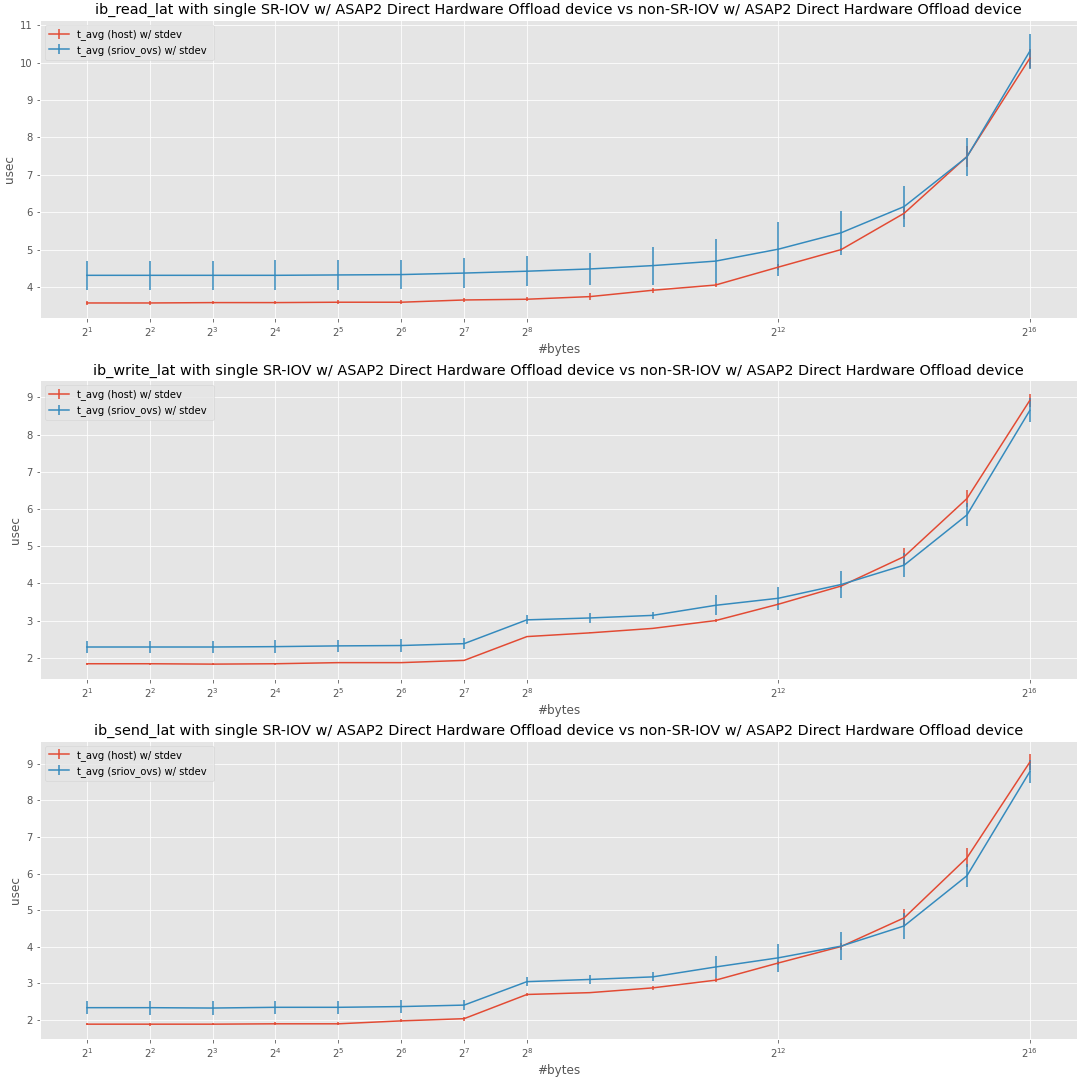
\includegraphics{asap2_direct_basic_lat.png}
	}
	\caption{Latency Tests}%
	\label{fig:asap2_direct_latency}
\end{figure}

\begin{figure}
	\centering
	\resizebox{0.8\linewidth}{!}{
		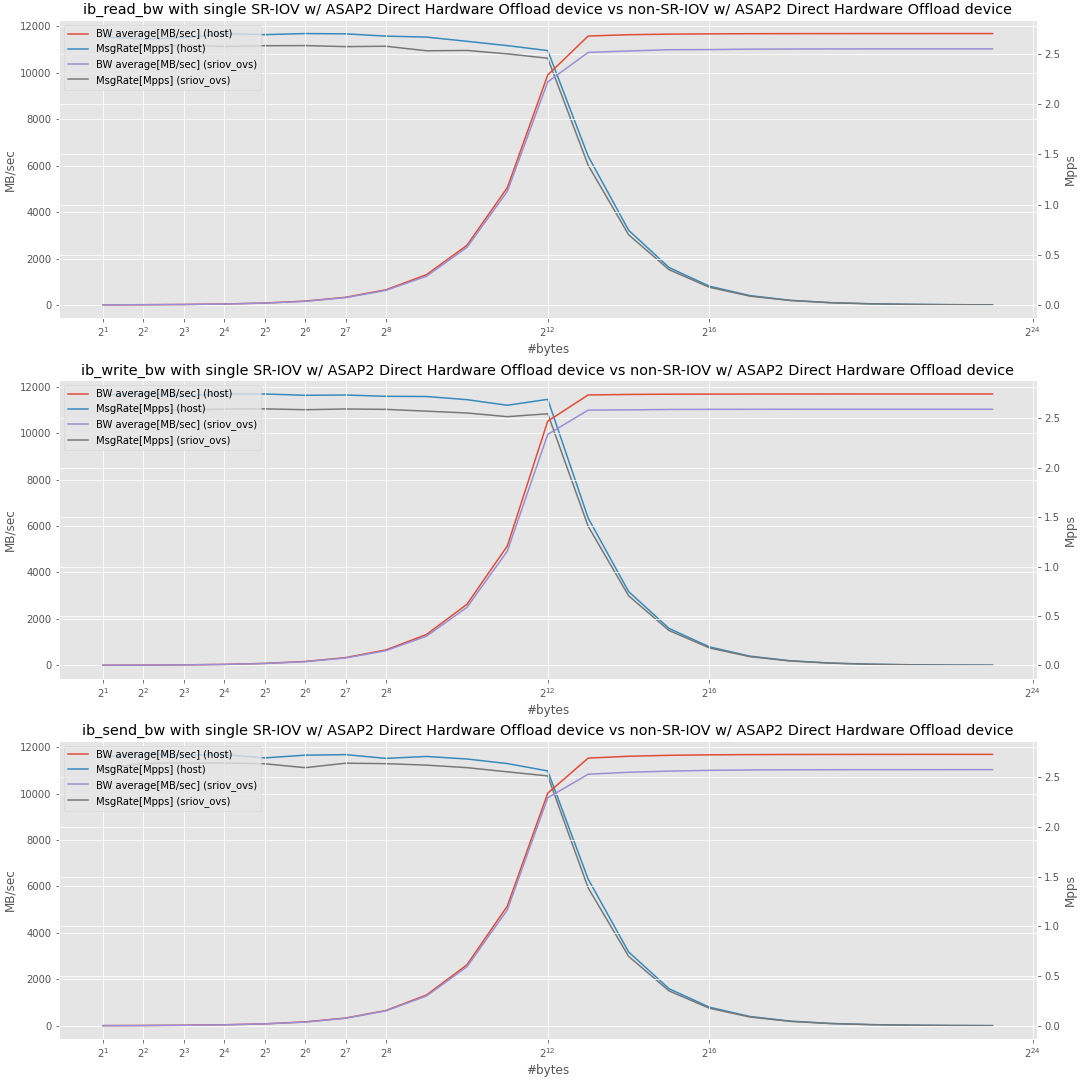
\includegraphics{asap2_direct_basic_bw.png}
	}
	\caption{Bandwidth Tests}%
	\label{fig:asap2_direct_bandwidth}
\end{figure}

\begin{figure}
	\centering
	\resizebox{0.8\linewidth}{!}{
		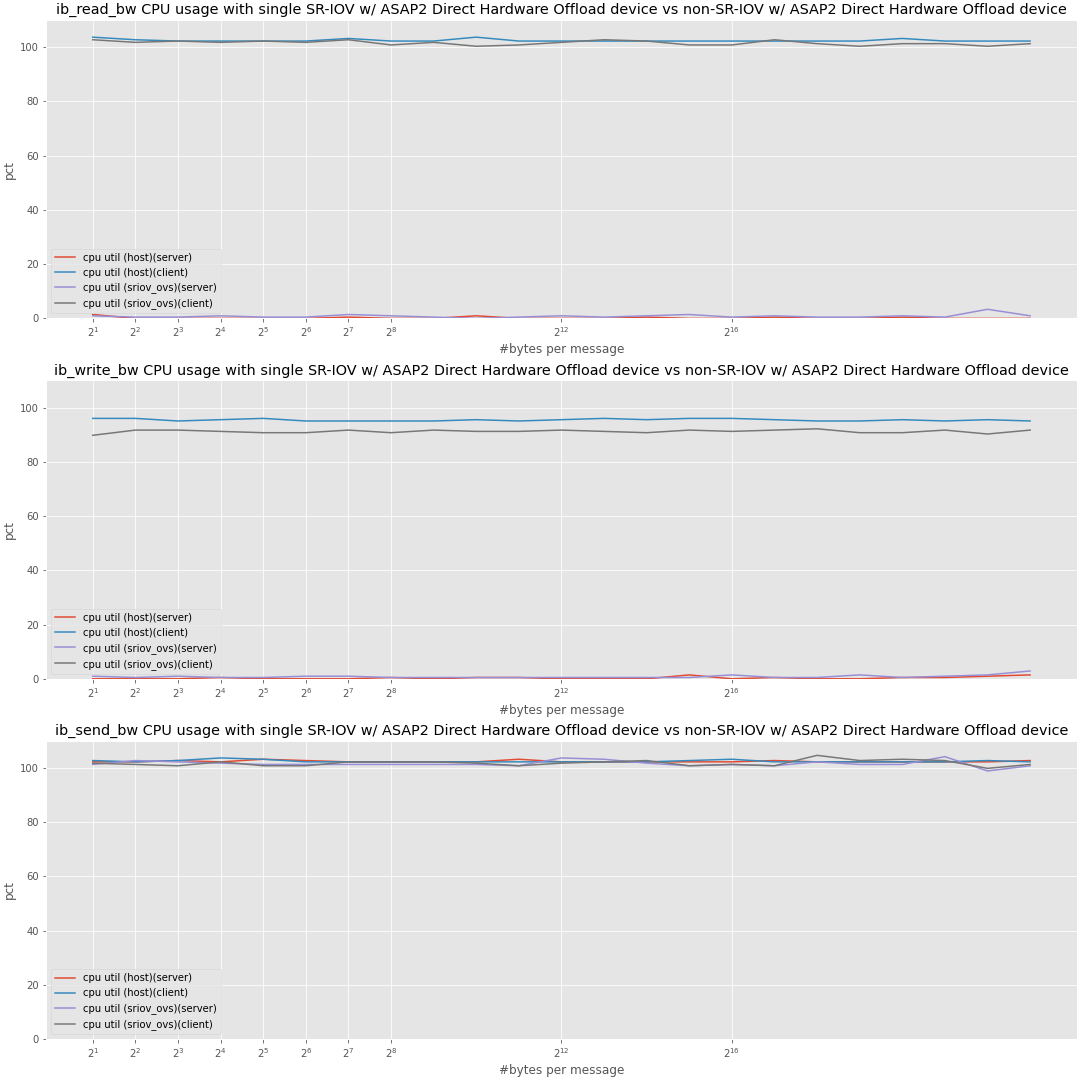
\includegraphics{asap2_direct_cpu.png}
	}
	\caption{CPU Utilization}%
	\label{fig:asap2_direct_cpu}
\end{figure}

Figures~\ref{fig:asap2_direct_latency},~\ref{fig:asap2_direct_bandwidth}, and~\ref{fig:asap2_direct_cpu} were all performed with either a single SR-IOV device (labeled \texttt{sriov\_ovs}) or a single raw RDMA device (labeled \texttt{host}), with varying RDMA message sizes.
Figure~\ref{fig:asap2_direct_latency} indicates that using ASAP$^2$ Direct has a noticeable latency overhead, more so than when just using SR-IOV alone. 
Interestingly, this latency overhead appears to disappear at large payloads, where it tended to increase with SR-IOV alone.
Figure~\ref{fig:asap2_direct_bandwidth} shows bandwidth results very similar to that of using SR-IOV alone, indicating perhaps that ASAP$^2$ Direct does not have much of an impact on bandwidth and the majority of that overhead comes from the use of SR-IOV.
Again, ss expected, Figure~\ref{fig:asap2_direct_cpu} shows CPU performance is not worse than when using the raw host RDMA device as all of the Open-VSwitch processing and NIC multiplexing is happening at the NIC and not at the CPU.

% todo: add multi dev tests

\subsubsection*{Miscellaneous Comments}
\begin{description}[nolistsep,font={{\scshape\bfseries}}]
	\item[Scalability Limits] unknown how many policies can be defined on a NIC at once
	\item[Proprietary] policy definitions are not proprietary, but policy execution is entirely proprietary and requires specialized Mellanox hardware
	\item[Maturity] unknown, but with heavy vendor support appears to be mature enough for production use
	\item[Ease in Deployment] requires integration with SR-IOV and specialized Open vSwitch policy definitions, not as easy to plug and play
	\item[Execution Privileges] requires no additional privileges
	\item[Network Pressure] no additional network pressure when used with SR-IOV
\end{description}


% How to test:
% Uninstall Mellanox OFED drivers (use ./uninstall.sh in MLNX_OFED)
% Install `rdma-core` and `perftest`
% Run `modprobe -rv mlx5_ib` and reboot.
% Bring up SoftRoCE RDMA devices with `rdma link`
% Disable RoCE on the underlying link (https://bugs.launchpad.net/ubuntu/+source/linux/+bug/1877270), this has to be done AFTER `rdma link`.
%
% Other links:
% https://github.com/linux-rdma/rdma-core/blob/master/Documentation/rxe.md
% https://community.mellanox.com/s/article/howto-configure-soft-roce


\subsection{Software Solutions: SoftRoCE}
SoftRoCE is a full software implementation of a RoCE-capable RDMA stack that can be used to create virtualized RDMA devices that run on top of existing Ethernet NICs~\cite{softroceoverview}. 
The ``fully in-software'' bit allows for total configuration of the virtualized RDMA device, which can be used to create fully isolated, virtualized RDMA devices that preserve and integrate with all container isolation systems.
However, it also come at the cost of massive performance penalties from: 
\begin{enumerate*}[label={(\arabic*)},itemjoin*={{, and }},itemjoin={{, }}]
	\item being unable to provide any hardware performance benefits from standard hardware RDMA devices
	\item requiring full software execution of the RDMA stack
	\item having to be run on top of the existing kernel TCP/UDP stack
\end{enumerate*}.
While some of these are optimized for with the SoftRoCE now being implemented as a kernel driver, SoftRoCE still remains a low performance RDMA solution~\cite{softrocedriver}.
Thus, SoftRoCE is likely viable only for specific niche use cases, such as for those who don't need the performance of RDMA and are simply seeking to enable RDMA compatibility (e.g.\ an RDMA client inside of a container).

\subsubsection*{Container Network Properties}
\begin{description}[nolistsep,font={{\scshape\bfseries}}]
	\item[Network Isolation] provides full container network isolation
	\item[Controllability] routing policies and traffic shaping are possible and fully configurable
	\item[Resource Utilization] requires significant CPU and memory to run the RDMA stack
\end{description}

\subsubsection*{Performance Tests}
All of the following tests were performed on Cloudlab with two d6515 hosts, which have a 32 core AMD 7452 at 2.35GHz CPU, 128GB RAM, and a dual port ConnectX--5 100 Gbit NIC~\cite{cloudlab}. 
Both were running Ubuntu 21.10 with Linux kernel version 5.13.0-35\footnote{Linux kernel version 5.8 on Ubuntu 20.04 appears to have a SoftRoCE bug that caused multiple kernel panics and was thus unusable.}, and were using the open source \texttt{rdma-core} and \texttt{perftest} packages.

\begin{figure}
	\centering
	\resizebox{0.8\linewidth}{!}{
		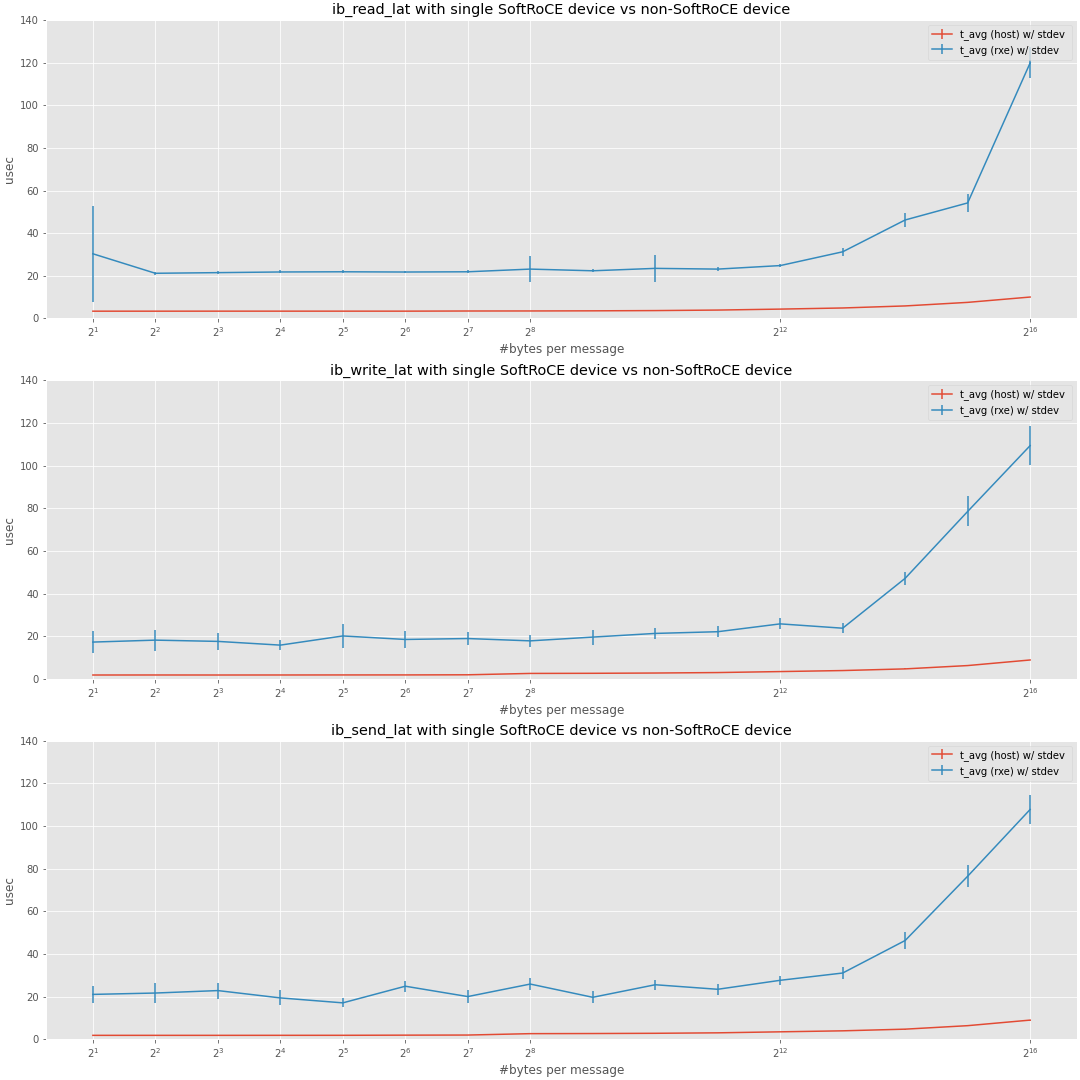
\includegraphics{softroce_basic_lat.png}
	}
	\caption{Latency Tests}%
	\label{fig:softroce_latency}
\end{figure}

\begin{figure}
	\centering
	\resizebox{0.8\linewidth}{!}{
		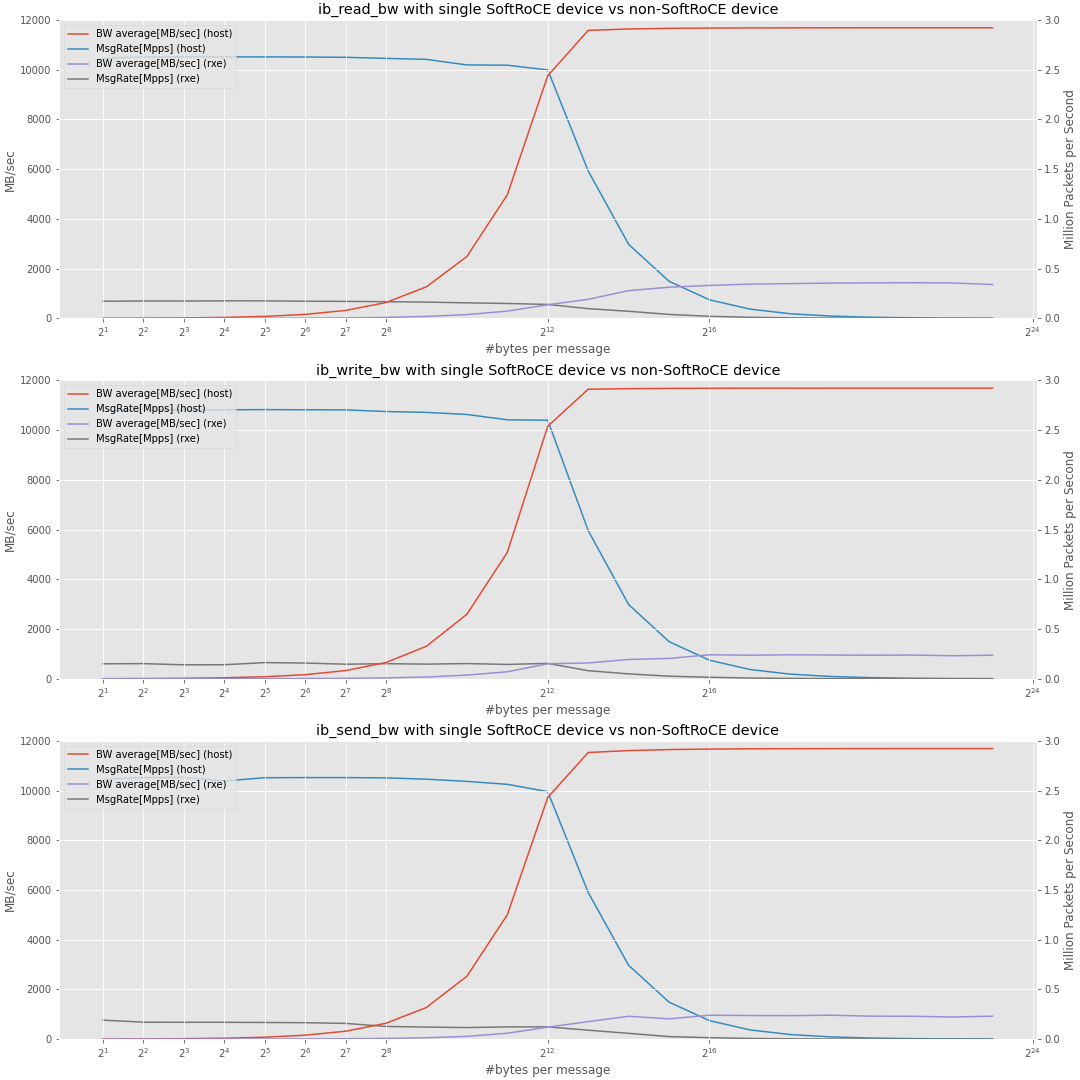
\includegraphics{softroce_basic_bw.png}
	}
	\caption{Bandwidth Tests}%
	\label{fig:softroce_bandwidth}
\end{figure}

\begin{figure}
	\centering
	\resizebox{0.8\linewidth}{!}{
		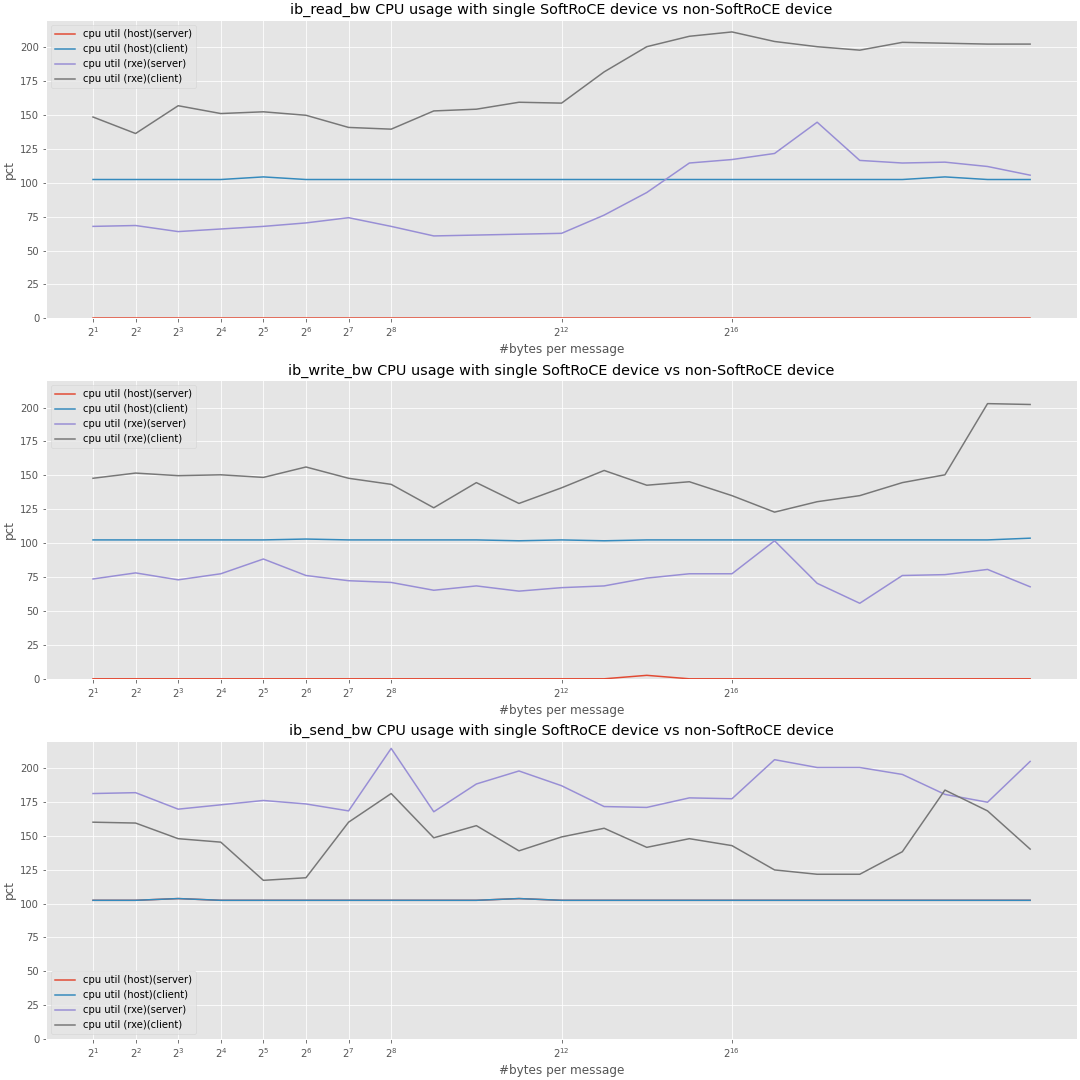
\includegraphics{softroce_cpu.png}
	}
	\caption{CPU Utilization}%
	\label{fig:softroce_cpu}
\end{figure}

Figures~\ref{fig:softroce_latency},~\ref{fig:softroce_bandwidth}, and~\ref{fig:softroce_cpu} were all performed with either a single SoftRoCE device (labeled \texttt{rxe}) or a single raw RDMA device (labeled \texttt{host}), with varying RDMA message sizes.
Figure~\ref{fig:softroce_latency} shows a significant increase in both latency and deviation in latency when compared to using a non-SoftRoCE device (the non-SoftRoCE device also has error bands, but they are so small they are imperceivable in the graph).
Figure~\ref{fig:softroce_bandwidth} highlights how a single SoftRoCE device has both a bandwidth and message rate potential that is significantly less than that of a non-SoftRoCE device. 
Figure~\ref{fig:softroce_cpu} shows the total CPU usage during an \texttt{ib\_read\_bw} test on both the client and server. 
Unsurprisingly, SoftRoCE usage resulted in more CPU utilization than a non-SoftRoCE device on the client. 
Furthermore, the total CPU usage across both the server and client is greater with a SoftRoCE device than on a non-SoftRoCE device, which is expected.
In normal RDMA, the server requires no CPU utilization (for one-sided operations) as the RDMA device itself handles that.
With SoftRoCE, the server has to spend CPU cycles processing incoming packets, resulting in higher CPU utilization.
One noticable feature about the CPU graphs is how SoftRoCE usage can result in a CPU utilization of 200\%. 
This is likely due to one CPU core being entirely used for SoftRoCE processing and one CPU core being entirely used for the actual \texttt{ib\_read\_bw} program.

\begin{figure}
	\centering
	\resizebox{0.8\linewidth}{!}{
		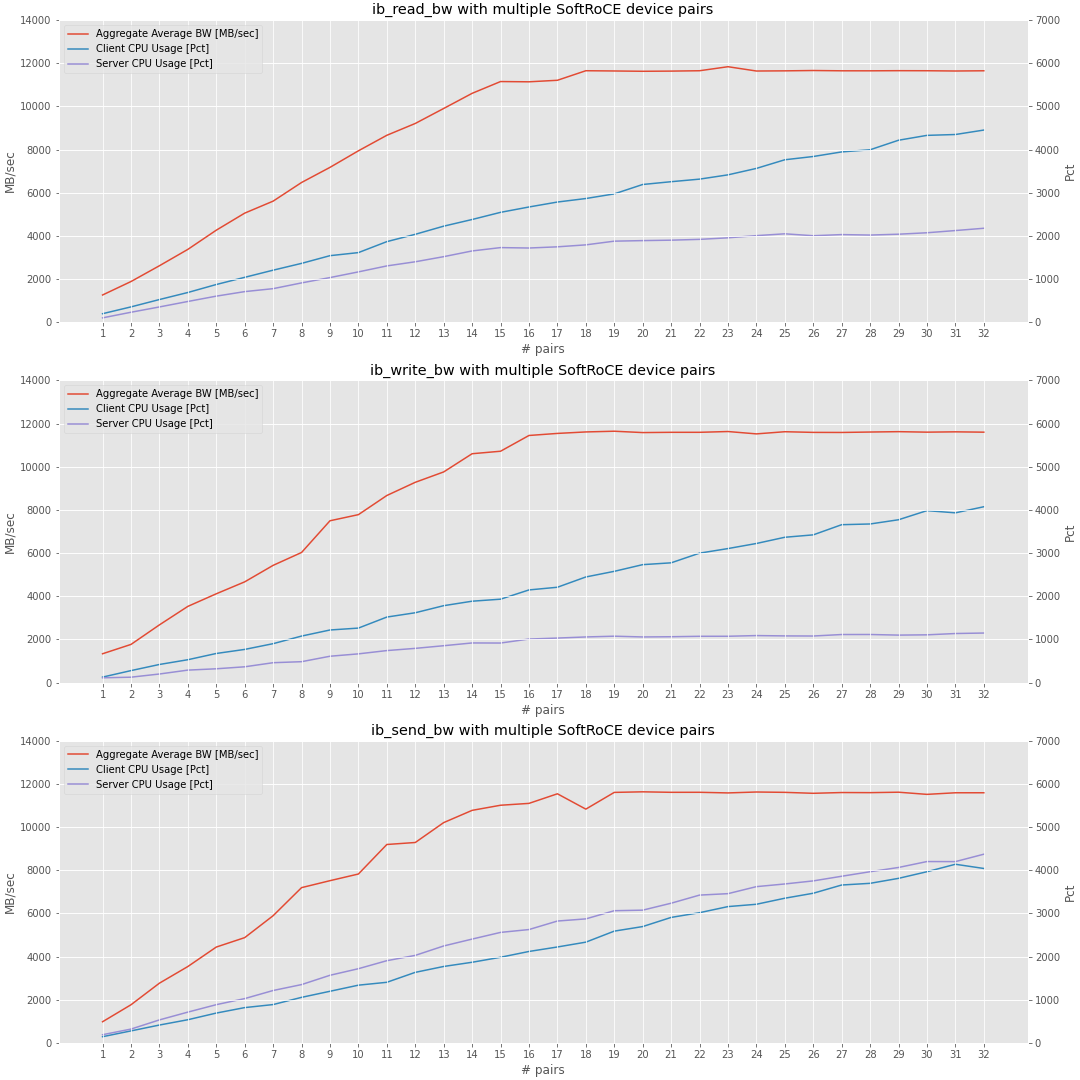
\includegraphics{softroce_multi_vdev.png}
	}
	\caption{Bandwidth + CPU with Multiple Devices}%
	\label{fig:softroce_multi_vdev}
\end{figure}

Figure~\ref{fig:softroce_multi_vdev} was performed with multiple SoftRoCE devices created on both the client and server, with a single \texttt{ib\_(read|write|send)\_bw} test running on each device with a byte size of 65536.
For each SoftRoCE device, a \texttt{macvlan} interface was created on the RDMA device's interface to serve as the SoftRoCE device's parent, which is necessary as an interface can only parent one SoftRoCE device.

This data highlights several things.
First, use of SoftRoCE alone appears to be capable of fully saturating the underlying NIC's bandwidth.
In this case, for \texttt{ib\_read\_bw}, it took approximately 18 pairs of SoftRoCE devices, approximately 30 CPU cores worth of CPU cycles on the server, and approximately 19 CPU cores worth of CPU cycles on the client to saturate the underlying NIC's bandwidth (i.e.\ match the bandwidth performance of the non-SoftRoCE device).
Second, even after saturating the underlying NIC's bandwidth, client CPU utilization continued to climb linearly with each additional SoftRoCE device.

All in all, these graphs highlight how SoftRoCE fails to match the bandwidth, latency, and CPU performance of a raw RDMA device, and is not desirable for use in performance sensitive environments.
SoftRoCE can scale to saturate the underlying NIC's bandwidth, but requires substantial CPU utilization which significantly hurts its scalability.

\subsubsection*{Miscellaneous Comments}
\begin{description}[nolistsep,font={{\scshape\bfseries}}]
	\item[Scalability Limits] cannot scale due to CPU contention
	\item[Proprietary] open source kernel driver that has been upstreamed, so it is available to all Linux users
	\item[Maturity] relatively mature, but has little development outside of the research community thus suffers from a number of bugs~\cite{softrocedriver}
	\item[Ease in Deployment] quick to deploy using standard \texttt{iproute2} tools
	\item[Execution Privileges] requires no additional privileges
	\item[Network Pressure] creates no additional network pressure than using standard networking
\end{description}

\section{Discussion}
\subsection{Security}
Security is often a concern among those adopting containers, especially when using containers to facilitate a multi-tenant environment.
Focusing on just RDMA for a minute, RDMA provides on-host security with the use of the RDMA management plane and cryptographic keys, as explained in Section~\ref{subsec:RDMA Protocol}.
The management plane ensures RDMA devices cannot be reconfigured without the proper permissions on the host and cryptographic keys provide a mechanism to ensure remote hosts cannot read arbitrary memory regions.
However, RDMA suffers from minimal network security as RDMA packets have no form of encryption, thus making RDMA vulnerable to eavesdropping, man-in-the-middle, and tampering attacks.
This is particularly a problem as RDMA packets contain the \texttt{pkey} --- the cryptographic key used to authorize access to remote memory regions --- in plaintext in the unencrypted RDMA packet.
If eavesdropped on, obtaining this \texttt{pkey} would allow outside actors to bypass all RDMA memory region restrictions~\cite{rdmasecurity}.

Solving this is non-trivial; encryption would require reading and rewriting the entirety of the RDMA packet. 
As RDMA bypasses the kernel and CPU, encryption would then have to be done on the RDMA NIC itself and, until recently, no NIC has provided this feature.
Given this, the use of RDMA in containers would inherit this security vulnerability and no RDMA in container solution would be able to solve this as it must be done at the NIC level.

For the security of the management plane for RDMA in container solutions, almost every solution inherits the security provided by the core RDMA protocol.
Some solutions, such as FreeFlow, would have to implement their own security model for the management of their virtual RDMA devices as only FreeFlow is aware of these devices.
For other solutions where the kernel is aware of the virtual devices, these solutions would piggyback on existing RDMA management plane security and their use would not open any potential security concerns.

Beyond the security vulnerabilities introduced by RDMA itself, use of these RDMA-in-container solutions do open a security hole if they do not provide true inter-host / network isolation.
Nearly all RDMA devices have been shown to have deterministic, or at the very least highly guessable, memory key generation algorithms~\cite{redmark}.
Thus, even if network operators limited the snooping ability of RDMA devices inside of containers, its possible for individual containers to guess the memory keys of remote hosts.
This would render multi-tenant environments with RDMA-in-container solutions extremely insecure.
Environments looking to use an RDMA-in-container solution in a multi-tenant environment are recommended to create full, network level isolation between each RDMA-in-container device to mitigate these issues.

\subsection{Network Reconfiguration}
One other potential solution for enabling RDMA-in-containers would be to use network reconfiguration, where the container network policies are enforced by the underlying network instead of by the host or NIC\@.
Alongside the use of SR-IOV, shared HCAs, or VLAN tagging, this could provide another fast, configurable, and low resource utilizing solution for RDMA-in-containers.
This would operate similar to existing container networking solutions like Project Calico using BGP~\cite{caliconetwork}.
With the variability in network configuration, types (e.g.\ Infiniband or Ethernet), privilege escalation risks (e.g.\ would the container orchestration software itself be able to reconfigure the network?), and available network resources, it is difficult to generalize properties of this solution thus is left for each environment to assess for themselves.

\subsection{Looking Forward}
It seems the future of RDMA in containers is converging toward a paravirtualization-like approach for intra-machine RDMA device isolation and a hardware-based approach for inter-machine RDMA device isolation.
In other words, paravirtualization --- likely in the form of kernel managed virtual RDMA devices with the NIC having some visibility into those --- would be used to create individual RDMA devices for each container.
Hardware offload would be used to enforce network policies for each of those virtual devices. 
This suggests that a true RDMA in container solution would require new, specialized NICs that have both hardware offload and paravirtualization support, meaning RDMA in containers would incur additional costs for new hardware and will not be possible on older, existing RDMA hardware. 

This comes, in part, from the direction and substantial investment Mellanox is making in this space.
Unfortunately, while projects like FreeFlow and MasQ are desirable from an accessibility perspective, they suffer from a number of problems.
First, much of the RDMA space is industry driven to begin with, especially given how complex and hardware specific the RDMA protocol and code base is.
It's difficult for non-industry driven solutions to remain relevant as they would have to continually pull and patch upstream changes in the RDMA protocol/code base, which is difficult to maintain.
Second, as shown by the data, purely in software approaches require substantial CPU sacrifices and suffer in scalability. 
This indicates that at least part of the RDMA in container solution must involve a form of hardware offload.
Third, for high performance computing environments, the security and support provided by vendor support solutions is unmatched when compared to small research projects like FreeFlow. 
It would seem obvious these environments should rely on vendor supported solutions for this reason alone.

In terms of what RDMA tooling will look like in this future, it does appear that the RDMA in container solution will integrate closely with existing container isolation tooling.
Management of paravirtualized RDMA devices is already possible using the \texttt{rdma} CLI from the \texttt{iproute2} package, similar to using the \texttt{ip} CLI for network namespace management, and support for the \texttt{rdma} CLI appears to be growing.


\section{Conclusion}
While containers are quickly 
If you can afford it, NICs with hardware support for container topologies seem to be the best option for flexibility, support, and performance.
You are at the mercy of Mellanox though.

The paravirtualized solutions seem like a good alternative, but they require a lot of maintenance to keep up to date, especially with how complex and industry-driven the RDMA code base is.

% while projects like FreeFlow are available to use now, and work as advertised, they don't seem the most stable and is not maintained, thus is likely unusable in production.

% while this isn't the most exciting of conclusions, it's likely that the best RDMA-in-container solution is going to be industry backed solutions

\section{Acknowledgments}
I would like to sincerely thank my thesis advisor, Dr.\ Ryan Stutsman, for all of his support in writing this thesis.
I would also like to thank Joe Breen at the University of Utah Center for High Performance Computing for all of his guidance in the space of containers and networking.

\section{Availability \& Reproducibility}
This thesis, all of the code used to run RDMA-in-container experiments, and the raw data collected from said experiments is open sourced and available at \newline\href{https://github.com/emersonford/thesis}{https://github.com/emersonford/thesis}.
All of the data produced for this thesis can be reproduced following the instructions listed in the Github repo's \texttt{README.md}.

\pagebreak
\printbibliography{}
% \nocite{*}
% \section*{References}
% \printbibliography[heading=subbibliography,keyword={containers},title={Containers}]{}
% \printbibliography[heading=subbibliography,keyword={containernetworking},title={Container Networking}]{}
% \printbibliography[heading=subbibliography,keyword={rdmacontainers},title={RDMA in Containers}]{}
% \printbibliography[heading=subbibliography,keyword={rdmaresearch},title={RDMA Specific Research}]{}
% \printbibliography[heading=subbibliography,keyword={highperfnetworking},title={High Performance Networking}]{}
% \printbibliography[heading=subbibliography,keyword={kernelbypassnetworking},title={Kernel Bypass Networking}]{}
% \printbibliography[heading=subbibliography,keyword={documentation},title={Documentation}]{}
% \printbibliography[heading=subbibliography,keyword={tutorial},title={Tutorials}]{}
% \printbibliography[heading=subbibliography,keyword={mellanox},title={Mellanox Infosheets}]{}

% \pagebreak
% \section*{Appendix}
% \appendix
\end{document}
